\documentclass{article}
\usepackage[]{graphicx}
\usepackage[]{xcolor}
\usepackage{alltt}
\usepackage[left=2.3cm,right=2.8cm, top = 2.2cm, bottom = 3cm]{geometry}
\usepackage{amsmath}
\usepackage{amssymb}
\usepackage{natbib}
\PassOptionsToPackage{hyphens}{url}
\usepackage{url} 
\usepackage[disable]{todonotes}
\usepackage{multicol}
\usepackage{rotating}
\usepackage{booktabs}
\usepackage[colorlinks=false]{hyperref} 
\setlength{\parskip}{\baselineskip}%
\setlength{\parindent}{0pt}%
\urlstyle{same}
\usepackage{lineno}
\linenumbers
\bibliographystyle{apalike}

% to handle authorship footnotes as numbers:
\makeatletter
\let\@fnsymbol\@arabic
\makeatother

\newcommand{\ra}[1]{\renewcommand{\arraystretch}{#1}}
\newcommand{\changed}[1]{#1}

% to write the simulated as iid symbol: 
\newcommand{\distas}[1]{\mathbin{\overset{#1}{\kern\z@\sim}}}%


\begin{document}



\title{Transformation of forecasts for evaluating predictive performance in an epidemiological context}
  \author{Nikos I. Bosse\thanks{Department of Infectious Disease Epidemiology, London School of Hygiene \& Tropical Medicine, London, United Kingdom} $^{,}$\thanks{Centre for the Mathematical Modelling of Infectious Diseases, London, United Kingdom} $^{,*}$, 
  Sam Abbott\footnotemark[1] $^{,}$\footnotemark[2]$ ^{}$, 
  Anne Cori\thanks{MRC Centre for Outbreak Analysis and Modelling, Department of Infectious Disease Epidemiology, School of Public Health, Imperial College London, London, United Kingdom} $^{}$, \\
  Edwin van Leeuwen\thanks{Department of Infectious Disease Epidemiology, London School of Hygiene \& Tropical Medicine, London, United Kingdom} $^{,}$\thanks{UK Health Security Agency, London, United Kingdom} $^{}$, 
  Johannes Bracher\thanks{Chair of Statistical Methods and Econometrics, Karlsruhe Institute of Technology, Karlsruhe, Germany}$^{,}$\thanks{Computational Statistics Group, Heidelberg Institute for Theoretical Studies, Heidelberg, Germany} $^{}$, 
  Sebastian Funk\footnotemark[1] $^{,}$\footnotemark[2]$ ^{}$}



\maketitle
%\tableofcontents
\begin{abstract}
Forecast evaluation plays an essential role in the development cycle of predictive epidemic models and can inform their use for public health decision-making. Common scores to evaluate epidemiological forecasts are the Continuous Ranked Probability Score (CRPS) and the Weighted Interval Score (WIS), which are both measures of the absolute distance between the forecast distribution and the observation. They are commonly applied directly to predicted and observed incidence counts, but it can be questioned whether this yields the most meaningful results given the exponential nature of epidemic processes and the several orders of magnitude that observed values can span over space and time. In this paper, we argue that transforming counts before applying scores such as the CRPS or WIS can effectively mitigate these difficulties and yield epidemiologically meaningful and easily interpretable results. We motivate the procedure threefold using the CRPS on log-transformed counts as an example: firstly, it can be interpreted as a probabilistic version of a relative error. Secondly, it reflects how well models predicted the time-varying epidemic growth rate. And lastly, using arguments on variance-stabilizing transformations, it can be shown that under the assumption of a quadratic mean-variance relationship, the logarithmic transformation leads to expected CRPS values which are independent of the order of magnitude of the predicted quantity. Applying the log transformation to data and forecasts from the European COVID-19 Forecast Hub, we find that it changes model rankings regardless of stratification by forecast date, location or target types. Situations in which models missed beginning upward swings are more strongly emphasized while failing to predict a downturn following a peak is less severely penalized. We conclude that appropriate transformations, of which the natural logarithm is only one particularly attractive option, should be considered when assessing the performance of different models in the context of infectious disease incidence. 

%Forecast evaluation plays an essential role in improving forecasting models and can support their role in informing decision-making. In epidemiology, probabilistic forecasts are often scored using the Weighted Interval Score (WIS) or the Continuous Ranked Probability Score (CRPS), which are measures of absolute distance between forecast and observation. Infectious disease transmission is commonly modelled as an exponential process characterized by the growth rate or the effective reproduction number. However, if the true objective of the forecaster is to predict future growth rates or reproduction numbers then scoring based on the absolute distance between forecast and observation may not reflect this underlying task well and thus make it difficult to compare forecasts across time, space, and forecast targets. As a solution, we propose transforming the data before scoring the forecasts to better reflect the underlying generative process. We further propose the natural logarithm  as a candidate transformation and discuss its interpretation as a measure of relative error and as a score for an implicit forecast of the exponential growth rate. Applying the natural logarithm to data from the European COVID-19 Forecast Hub, we found that it changed model rankings, regardless of stratification by forecast date, location or target types, and emphasised situations in which models missed lower inflection points and consequent rises in numbers, while penalising missed peaks less severely. We conclude that appropriate transformations, of which the natural logarithm is only one possible option, should be considered when assessing the performance of different models in the context of infectious disease incidence. 
\end{abstract}

\bigskip

{\footnotesize $^*$ Correspondence to \url{nikos.bosse@lshtm.ac.uk})}



\newpage


% ===========================================================
\section{Introduction}

Probabilistic forecasts \citep{heldProbabilisticForecastingInfectious2017} play an important role in decision-making in epidemiology and public health \citep{reichCollaborativeMultiyearMultimodel2019, funkShorttermForecastsInform2020, cramerEvaluationIndividualEnsemble2021, bracherShorttermForecastingCOVID192021, europeancovid-19forecasthubEuropeanCovid19Forecast2021, sherrattPredictivePerformanceMultimodel2022}, as well as other areas as diverse as economics \citep{timmermannForecastingMethodsFinance2018, elliottForecastingEconomicsFinance2016} or meteorology \citep{gneitingWeatherForecastingEnsemble2005, kukkonenReviewOperationalRegionalscale2012}. Epidemiological modelling in particular has received widespread attention during the COVID-19 pandemic. Evaluations of forecasts can provide feedback for researchers to improve their models and train ensembles. It moreover helps decision-makers distinguish good from bad predictions and choose forecasters (used here and elsewhere in this manuscript to mean anyone or anything that issues a forecast) and models that should inform future decisions.

Probabilistic forecasts are usually evaluated using so-called proper scoring rules \citep{gneitingStrictlyProperScoring2007}, which return a numerical score as a function of the forecast and the observed data. Proper scoring rules are constructed such that forecasters are incentivised to report their true belief about the future. Examples of proper scoring rules that have been used to assess epidemiological forecasts are the Continuous Ranked Probability Score~\citep[CRPS,][]{gneitingStrictlyProperScoring2007} or its discrete equivalent, the Ranked Probability Score~\citep[RPS,][]{funkAssessingPerformanceRealtime2019}, and the Weighted Interval Score \citep{bracherEvaluatingEpidemicForecasts2021}. 
The CRPS measures the distance of the predictive distribution to the observed data as 
\begin{linenomath*}
\begin{equation*}
    \text{CRPS}(F, y) = \int_{-\infty}^\infty \left( F(x) - 1(x \geq y) \right)^2 dx,
\end{equation*}    
\end{linenomath*}
where $y$ is the true observed value and $F$ the cumulative distribution function (CDF) of the predictive distribution. The CRPS can be understood as a generalisation of the absolute error to predictive distributions, and interpreted n the natural scale of the data. The WIS is an approximation of the CRPS for predictive distributions represented by a set of predictive quantiles and is currently used to assess forecasts in COVID-19 Forecast Hubs in the US \citep{cramerCOVID19ForecastHub2020, cramerEvaluationIndividualEnsemble2021}, Europe \citep{sherrattPredictivePerformanceMultimodel2022}, Germany and Poland \citep{bracherShorttermForecastingCOVID192021, bracherNationalSubnationalShortterm2021}, as well as the US Influenza Forecasting Hub \citep{CdcepiFlusightforecastdata2022}. The WIS is defined as 
\begin{linenomath*}
\begin{equation*}
    \text{WIS}(F, y) = \frac{1}{K} \times \sum_{k = 1}^{K} 2 \times \left[ \boldsymbol{1}(y \leq q_{\tau_k}) - \tau_k \right] \times ( q_{\tau_k} - y), 
\end{equation*}
\end{linenomath*}
where $q_{\tau}$ is the $\tau$ quantile of the forecast $F$, $y$ is the observed outcome, $K$ is the number of predictive quantiles provided and $\boldsymbol{1}$ is the indicator function. The WIS can be decomposed into three components, dispersion, overprediction, underprediction, which reflect the width of the forecast and whether it was centred above or below the observed value. We show an alternative definition based on central prediction intervals in Section \ref{sec:alternative-wis} which illustrates this decomposition more clearly. 

The dynamics of infectious processes are often described by the complementary concepts of the reproduction number $R$ \citep{gosticPracticalConsiderationsMeasuring2020} and growth rate $r$ \citep{wallingaHowGenerationIntervals2007}, where $R$ describes the strength and $r$ the speed of epidemic growth \citep{dushoffSpeedStrengthEpidemic2021}.
In the absence of changes in immunity, behaviour or other factors that may affect the intensity of transmission, the reproduction number would be expected to remain approximately constant.
In that case, the number of new infections in the population grows exponentially in time.
This behaviour was observed, for example, early in the COVID-19 pandemic in many countries~\citep{pellisChallengesControlCOVID192021}.

If case numbers are evolving based on an exponential process and the  modelling task revolves around estimating the reproduction number or the corresponding growth rate, then evaluating forecasts based on the absolute distance between forecast and observed value penalises underprediction (of the reproduction number or growth rate) less than overprediction by the same amount. This is because for exponential processes errors on the observed value grow exponentially with the error on the estimated reproduction number or growth rate. 
If one is to measure the ability of forecasts to assess and forecast the underlying infection dynamics, it may thus be more desirable to evaluate errors on the growth rate directly.

Evaluating forecasts using the CRPS or WIS means that scores represent a measure of absolute errors. However, forecast consumers may find errors on a relative scale easier to interpret and more useful in order to track predictive performance across targets of different orders of magnitude. 
\cite{bolinLocalScaleInvariance2021} have proposed the scaled CRPS (SCRPS) which is locally scale invariant; however, it does not correspond to a relative error measure and lacks a straightforward interpretation as available for the CRPS. 

A closely related aspect to relative scores (as opposed to absolute scores) is that in the evaluation one may wish to give similar weight to all considered forecast targets. As the CRPS typically scales with the order of magnitude of the quantity to be predicted, this is not the case for the CRPS, which will typically assign higher scores to forecast targets with high expected values (e.g., in large locations or around the peak of an epidemic). \cite{bracherEvaluatingEpidemicForecasts2021} have argued that this is a desirable feature, directing attention to situations of particular public health relevance. An evaluation based on absolute errors, however, will assign little weight to other potentially important aspects, such as the ability to correctly predict future upswings while observed numbers are still low. 

In many fields, it is common practice to forecast transformed quantities (see e.g. \cite{taylorEvaluatingVolatilityInterval1999} in finance, \cite{mayrLogLevelVAR2015} in macroeconomics, \cite{loweStochasticRainfallrunoffForecasting2014} in hydrology or \cite{fuglstadDoesNonstationarySpatial2015} in meteorology). While the goal of the transformations is usually to improve the accuracy of the predictions, they can also be used to enhance and complement the evaluation process. 
In this paper, we argue that the aforementioned issues with evaluating forecasts based on measures of absolute error can be addressed by transforming the forecasts and observations prior to scoring using some strictly monotonic transformation. Strictly monotonic transformations can shift the focus of the evaluation in a way that may be more appropriate for epidemiological forecasts, while preserving the propriety of the score. Many different transformations may be appropriate and useful, depending on the exact context, the desired focus of the evaluation, and specific aspects of the forecasts that forecast consumers care most about (see a broader discussion in Section \ref{sec:discussion}). 

For conceptual clarity and to allow for a more in-depth discussion, we focus mostly on the natural logarithm as a particular transformation (referred to as the log-transformtation in the remainder of this manuscript) in the context of epidemic phenomena. Instead of a score representing the magnitude of absolute errors, applying a log-transformation prior to the CRPS yields a score which a) measures relative error (see Section \ref{sec:methods:relative}), b) provides a measure for how well a forecast captures the exponential growth rate of the target quantity (see Section \ref{sec:methods:growthrate}) and c) is less dependent on the expected order of magnitude of the quantity to be predicted (see Section \ref{sec:methods:vst}). %The interpretation of the log-transformed score as a score for a forecast of the exponential growth rate of a given quantity aligns the evaluation with our understanding of how epidemiological processes should be modeled and the kinds of errors models would typically make. 
We therefore argue that such evaluations on the logarithmic scale should complement the prevailing evaluations on the natural scale. 
Other transformations may likewise be of interest. We briefly explore the square root transformation as an alternative transformation. %[and population standardization?]. 
Our analysis mostly focuses on the CRPS (or WIS) as an evaluation metric for probabilistic forecasts, given its widespread use throughout the COVID-19 pandemic. 

The remainder of the article is structured as follows. In Sections \ref{sec:methods:relative}--\ref{sec:methods:vst} we provide some mathematical intuition on applying the log-transformation prior to evaluating the CRPS, highlighting the connections to relative error measures, the epidemic growth rate and variance stabilizing transformations.
%We first provide a mathematical intuition of the impact of the log-transformation and its interpretation as relative error (Section \ref{sec:methods:relative}, measure of the accuracy of a forecast of the growth rate (Section \ref{sec:methods:growthrate}) and it's effect as a variance-stabilising transformation that makes can make scores independent of the mean of the forecast target (Section \ref{sec:methods:vst}. 
We then discuss practical considerations for applying transformations in general and the log-transformation in particular (Section \ref{sec:methods:considerations}) and the effect of the log-transformation on forecast rankings (section \ref{sec:methods:rankings}. To analyse the real-world implications of the log-transformation we use forecasts submitted to the European COVID-19 Forecast Hub  \citep{europeancovid-19forecasthubEuropeanCovid19Forecast2021, sherrattPredictivePerformanceMultimodel2022}. Finally, we provide scoring recommendations, discuss alternative transformations that may be useful in different contexts, and suggest further research avenues (Section \ref{sec:discussion}). 


%%%%%%%%%%%%%%%%%%%%%%%%%%%%%%%%%%%%%%%%%%%%%%%%%%%%%%%%%%%%%%%%%%%%%%%%%%%%
\section{Transforming forecasts and observations}
\label{sec:methods}

\subsection{Interpretation as a relative error}
\label{sec:methods:relative}

To illustrate the effect of applying the natural logarithm prior to evaluating forecasts we consider the absolute error, which the CRPS and WIS generalize to probabilistic forecasts. We assume strictly positive support (meaning that no specific handling of zero values is needed), a restriction we will address when applying this transformation in practice. When considering a point forecast $\hat{y}$ for a quantity of interest $y$, such that 
%
\begin{linenomath*}
\begin{equation*}
y = \hat{y} + \varepsilon,
\end{equation*}
\end{linenomath*}
the absolute error is given by $|\varepsilon|$. When taking the logarithm of the forecast and the observation first, thus considering 
\begin{linenomath*}
\begin{equation*}
\log y = \log \hat{y} + \varepsilon^*,
\end{equation*}
\end{linenomath*}
the resulting absolute error $\left|\varepsilon^*\right|$ can be interpreted as an approximation of various common relative error measures. Using that $\log(a) \approx a - 1$ if $a$ is close to 1, we get
$$
|\varepsilon^*| = |\log \hat{y} - \log y| = \left|\log\left(\frac{\hat{y}}{y}\right) \right| \ \ \stackrel{\text{if } \hat{y} \ \approx \ y}{\approx} \ \ \left| \frac{\hat{y}}{y} - 1 \right| \ \ = \ \ \left| \frac{\hat{y} - y}{y} \right|.
$$
The absolute error after log transforming is thus an approximation of the \textit{absolute percentage error} \citep[APE,][]{gneitingMakingEvaluatingPoint2011a}. As we assumed that $\hat{y} \approx y$, we can also interpret it as an approximation of the \textit{relative error} (RE)
$$
\left| \frac{\hat{y} - y}{\hat{y}} \right|
$$
and the \textit{symmetric absolute percentage error} (SAPE)
$$
\left| \ \frac{\hat{y} - y}{y/2 + \hat{y}/2} \ \right|.
$$
As Figure \ref{fig:SAPE} shows, the alignment with the SAPE is in fact the closest and holds quite well even if predicted and observed value differ by a factor of two or three. Generalising to probabilistic forecasts, the CRPS applied to log-transformed forecasts and outcomes can thus be seen as a probabilistic counterpart to the symmetric absolute percentage error, which offers an appealing intuitive interpretation.

\begin{figure}[h!]
\centering
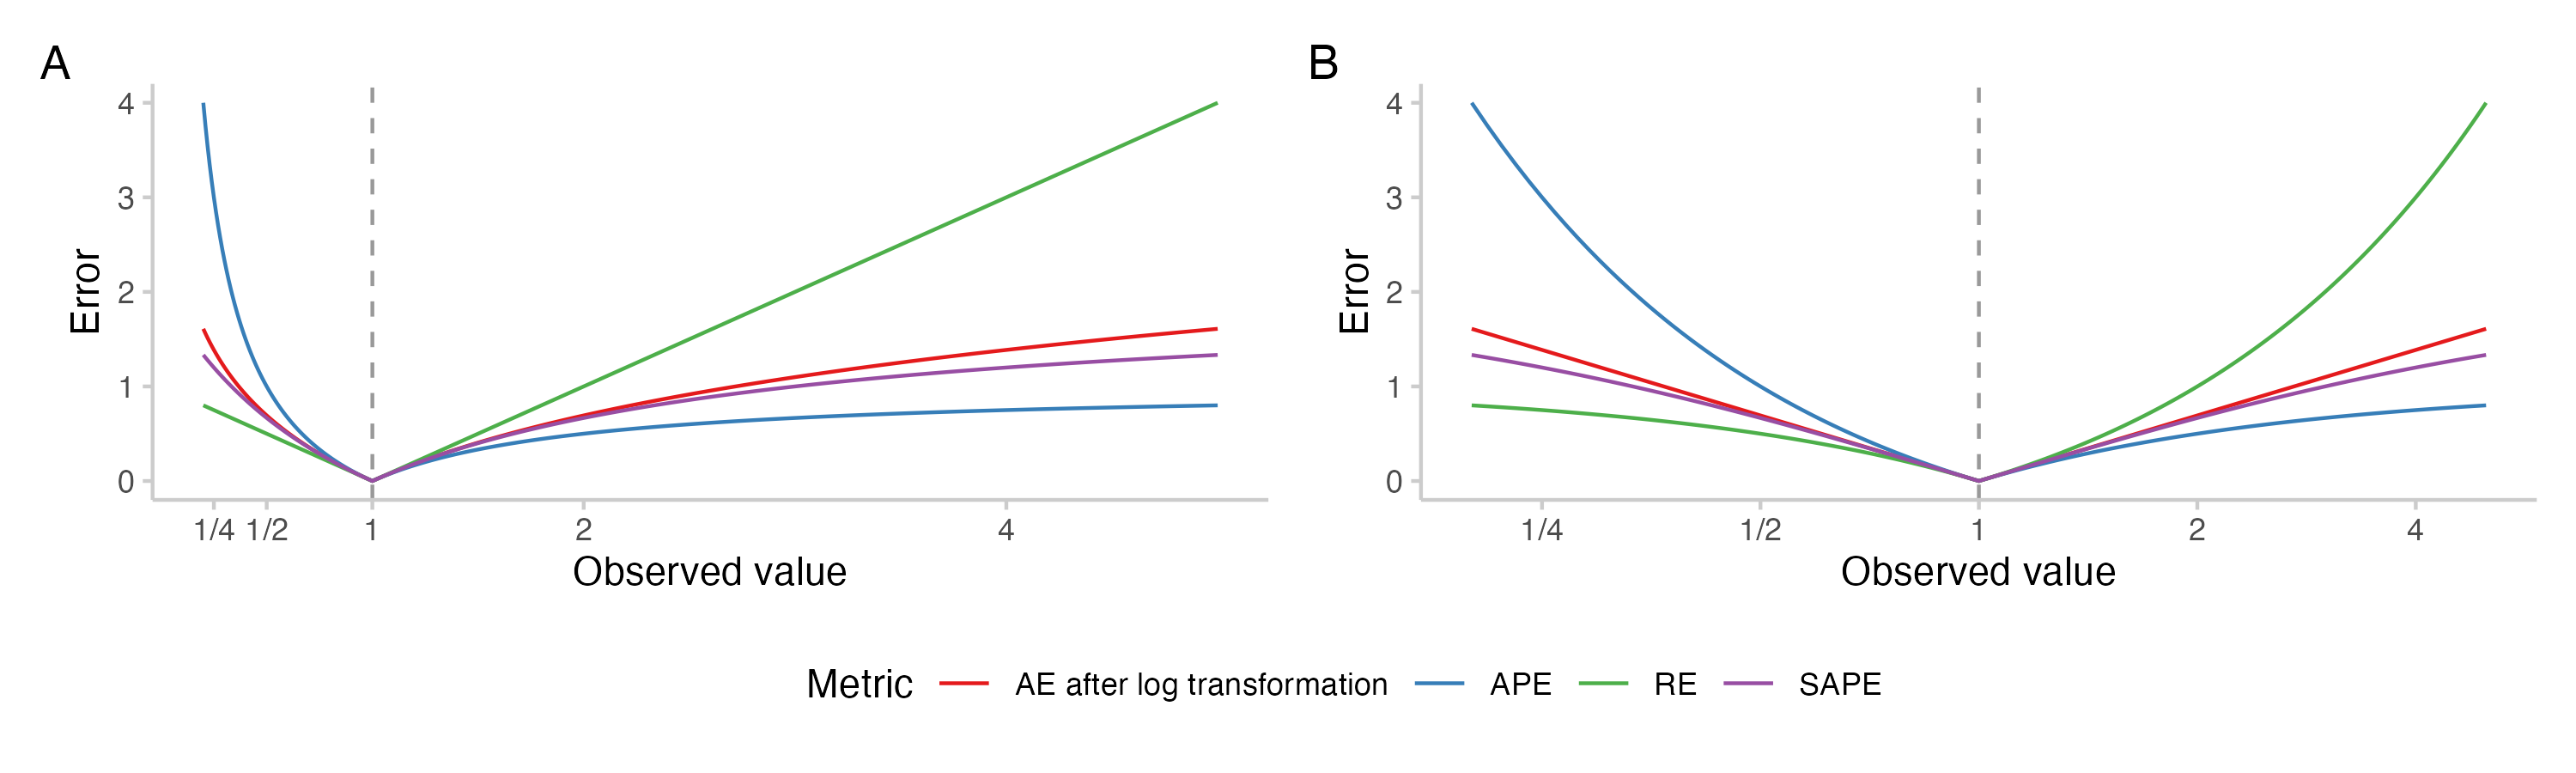
\includegraphics[width = 1\textwidth]{output/figures/different-relative-errors.png}
\caption{Numerical comparison of different measures of relative error: absolute percentage error (APE), relative error (RE), symmetric absolute percentage error (SAPE) and the absolute error applied to log-transformed predictions and observations. We denote the predicted value by $\hat{y}$ and display errors as a function of the ratio of observed and predicted value. A: x-axis shown on a linear scale. B: x-axis shown on a logarithmic scale.}
\label{fig:SAPE}
\end{figure}


%The analogy between the WIS on the log scale and the absolute error of a point forecast on the log scale is slightly inaccurate: while the absolute error on the log scale is exactly symmetric (e.g., predicting 2 instead of 1 would give the same relative error as predicting 0.5), this is not entirely true for the WIS, which is computed for a set of prediction intervals. Due to the fact that upper and lower bounds of individual prediction intervals are affected slightly differently by the log-transformations, small deviations may occur (compare e.g. in Figure \ref{fig:change-in-scores}D the small difference between scores for an observed outcome of $\frac{1}{5}$ and 5). 



\subsection{Interpretation as scoring the exponential growth rate}
\label{sec:methods:growthrate}

Another interpretation for the log-transform is possible if the generative process is framed as exponential with a time-varying growth rate $r(t)$~\citep[see, e.g.,][]{wallingaHowGenerationIntervals2007}, i.e.
\begin{linenomath*}
\begin{equation*}
\frac{d}{dt}y(t) = r(t)y(t)
\end{equation*}
\end{linenomath*}
%
which is solved by
%
\begin{linenomath*}
\begin{equation*}
y(t) = y_0 \exp \left( \int_0^t r(t') dt' \right) = y_0 \exp (\bar{r}t)
\end{equation*}
\end{linenomath*}
where $y_0$ is an initial data point and $\bar{r}$ is the mean of the growth rate between the initial time point $0$ and time $t$.

If a forecast $\hat{y}(t)$ for the value of the time series at time $t$ is issued at time 0 based on the data point $y_0$ then the absolute error after log transformation is
%
\begin{linenomath*}
\begin{align*}
\epsilon^* &= \left| \log \left[ \hat{y}( t ) \right] - \log \left[ y ( t ) \right] \right|\\
           &= \left| \log \left[ y_0 \exp (\bar{\hat{r}} t ) \right] - \log \left[ y_0 \exp (\bar{r}t) \right] \right|\\
           &= t \left| \bar{\hat{r}} - \bar{r} \right|
\end{align*}
\end{linenomath*}
%
where $\bar{\hat{r}}$ is the true mean growth rate and $\bar{r}$ is the forecast mean growth rate. We thus evaluate the error in the mean exponential growth rate, scaled by the length of the time period considered. Again generalising this to the CRPS and WIS implies a probabilistic evaluation of forecasts of the epidemic growth rate.

\subsection{Interpretation as a variance-stabilising transformation}
\label{sec:methods:vst}

When evaluating models across sets of forecasting tasks, it may be desirable for each target to have a similar impact on the overall results. In disease forecasting, this is not the case when using the CRPS, as the latter typically scales with the order of magnitude of the quantity to be predicted. Average scores are then dominated by the results achieved for targets with high expected outcomes. 
%Bracher et al. mention this as a desirable feature of the CRPS. 
% In epidemiological contexts, the variance of the variable of interest usually scales with its mean. 
Specifically, if the predictive distribution for the quantity $Y$ equals the true data-generating process $F$ (an ideal forecast), the expected CRPS is given by \citep{gneitingStrictlyProperScoring2007}
$$
\mathbb{E}[\text{CRPS}(F, y)] = 0.5\times\mathbb{E}|Y - Y'|,
$$
where $Y$ and $Y'$ are independent samples from $F$. This corresponds to half the \textit{mean absolute difference}, which is a measure of dispersion. If $F$ is well-approximated by a normal distribution $\text{N}(\mu, \sigma^2)$, the approximation
$$
\mathbb{E}_F[\text{CRPS}(F, y)] \approx \frac{\sigma}{\sqrt{\pi}}
$$
can be used. This means that the expected CRPS scales roughly with the standard deviation, which in turn typically increases with the mean in epidemiological forecasting. In order to make the expected CRPS independent of the expected outcome, a \textit{variance-stabilising transformation} \citep[VST,][]{bartlettSquareRootTransformation1936} can be employed. The choice of this transformation depends on the mean-variance relationship of the underlying process. 

If the mean-variance relationship is quadratic with $\sigma^2 = c \times \mu^2$, the natural logarithm can serve as the VST \citep{guerreroTimeseriesAnalysisSupported1993}. Denoting by $F_{\log}$ the predictive distribution for $\log(Y)$, we can use the delta method to show that
$$
\mathbb{E}_F[\text{CRPS}\{F_{\log}, \log(y)\}] \approx \frac{\sigma/\mu}{\sqrt{\pi}} 
= \frac{\sqrt{c}}{\sqrt{\pi}}
.
$$
The assumption of a quadratic mean-variance relationship is closely linked to the aspects discussed in Sections \ref{sec:methods:relative} and \ref{sec:methods:growthrate}. It implies that relative errors have constant variance and can thus be meaningfully compared across different targets. Also, it arises naturally if we assume that our capacity to predict the epidemic growth rate does not depend on the expected outcome.

If the variance is linear with $\sigma^2 = c \times \mu$, as with a Poisson-distributed variable, the square root is known to be a VST. 
Denoting by $F_{\sqrt{\ }}$ the predictive distribution for $\sqrt{Y}$, the delta method can again be used to show that
$$
\mathbb{E}_F[\text{CRPS}\{F_{\sqrt{\ }}, \sqrt{y}\}] \approx \frac{\sigma/\sqrt{\mu}}{2\sqrt{\pi}} = \frac{\sqrt{c}}{2\sqrt{\pi}}
.
$$

% which one is an empirical question - maybe hint that quadratic may result from RW on growth rate?

To strengthen our intuition on how transforming outcomes prior to applying the CRPS shifts the emphasis between targets with high and low expected outcomes, Figure \ref{fig:SIM-wis-state-size-mean} shows the expected CRPS of ideal forecasters under different mean-variance relationships and transformations. We consider a Poisson distribution where $\sigma^2 = \mu$, a geometric distribution where $\sigma^2 = \mu + \mu^2$, and a negative binomial distribution where the size parameter $\psi(\mu)$ depends on the mean $\mu$ such that $\sigma^2 = \mu + \mu^{2.5}/1000$. We see that when applying the CRPS on the natural scale, the expected CRPS grows in $\mu$ in all cases. When applying it after a log-transformation, the expected CRPS is almost independent of $\mu$ for the geometric distribution and large $\mu$, while smaller targets have higher expected CRPS in the Poisson case. When applying a square-root-transformation before the CRPS, the expected CRPS is independent of the mean for the Poisson-distribution and grows for the two other distributions. 
%For the negative binomial distribution, targets with very small and very high expectation yield the highest expected CRPS. \textbf{Here it would be nice to also add a sentence on what happens under sqrt transformation.} % scores are independent of the mean of the forecast target. For a Poisson-distribution with 
% $\sigma = \mu$, scores on the log scale decrease as the mean increases. The appropriate variance-stabilising transformation here to make scores independent of the mean would be a square-root-transformation . 

\begin{figure}[h!]
    \centering
    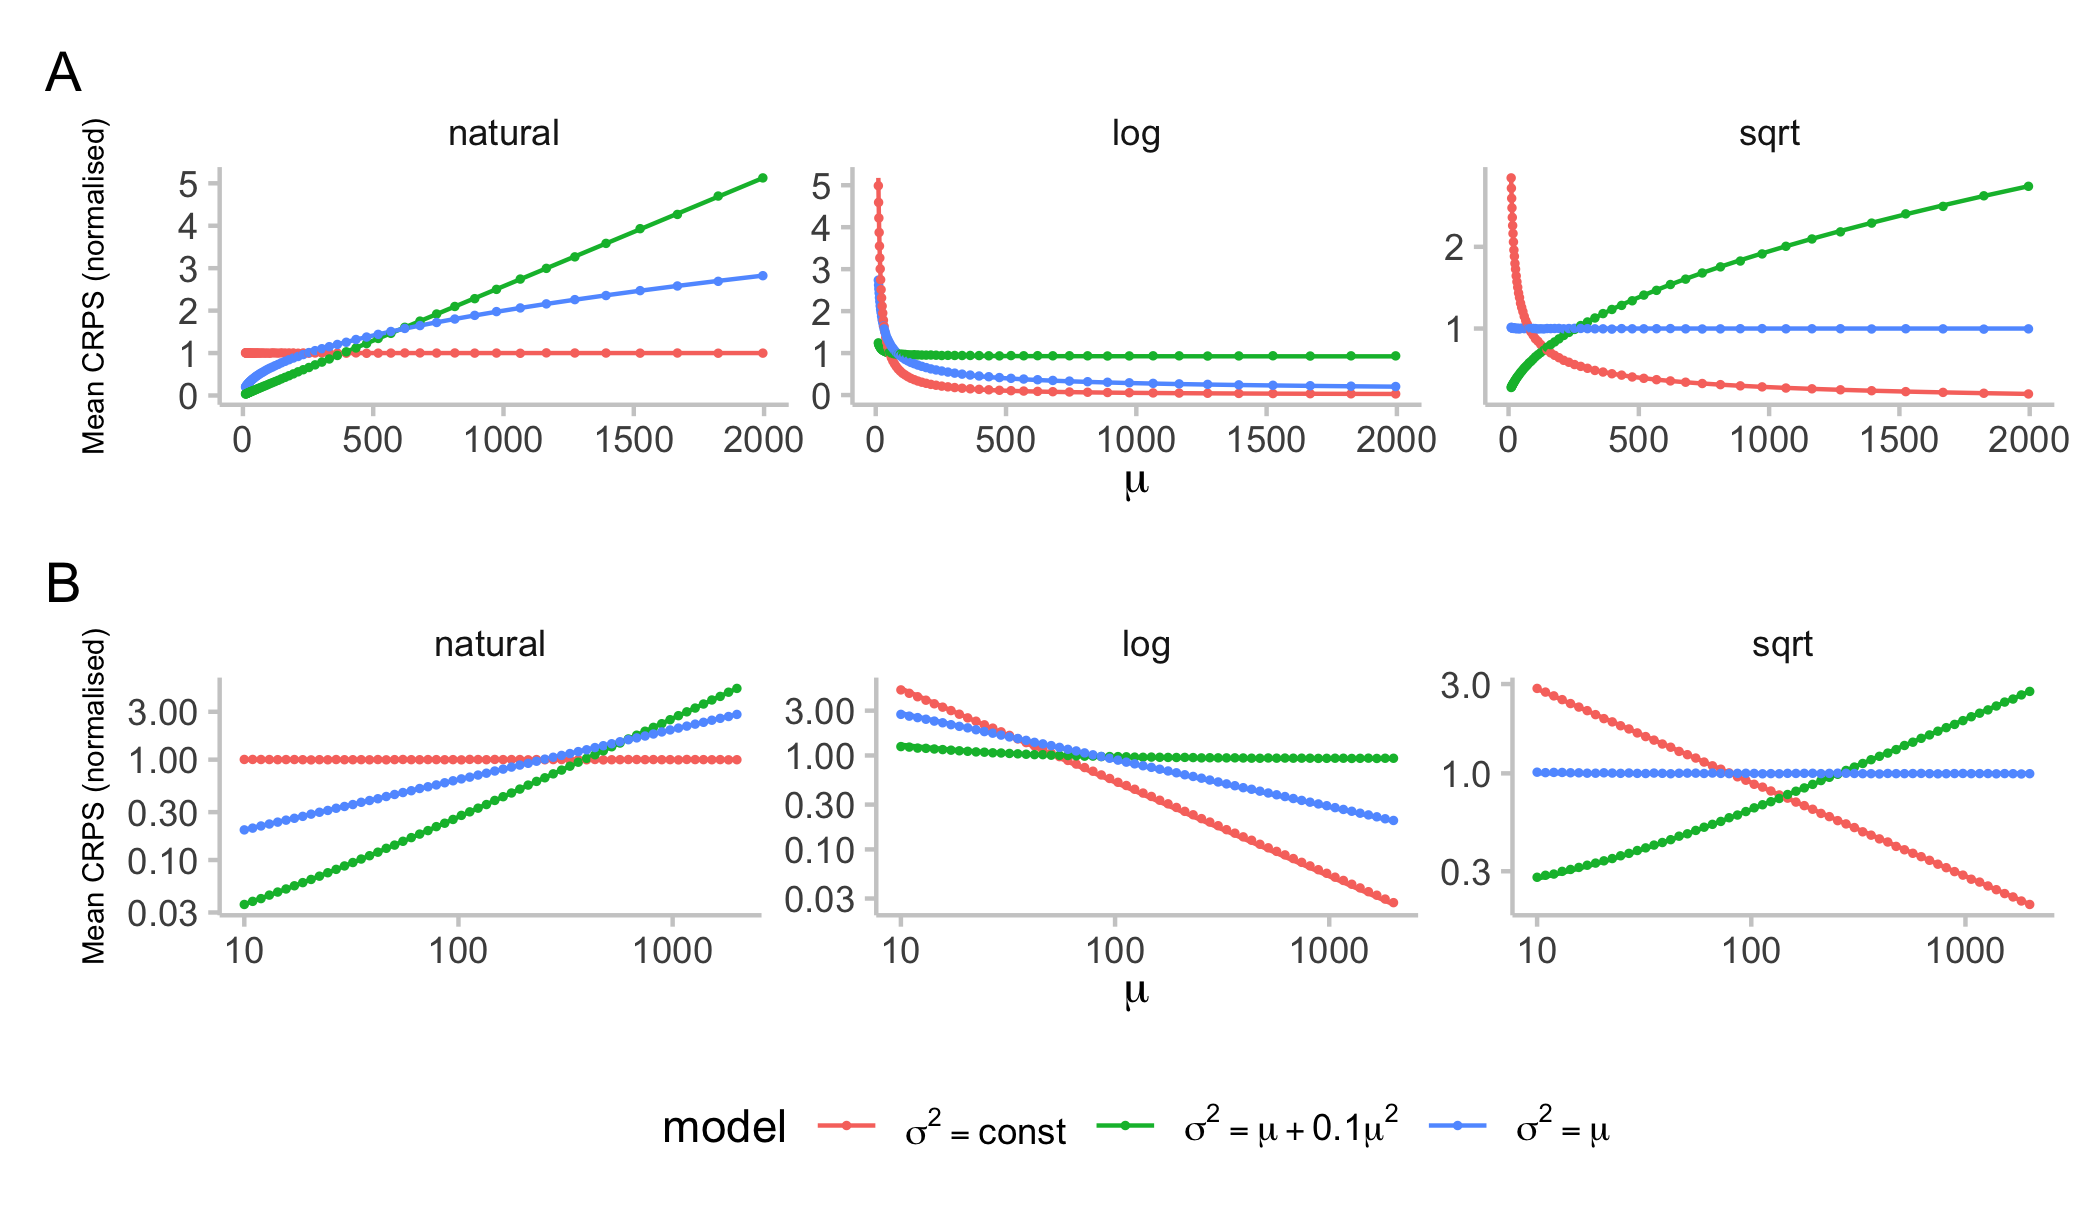
\includegraphics[width=0.99\textwidth]{output/figures/SIM-mean-state-size.png}
    \caption{Expected CRPS scores as a function of the mean and variance of the forecast quantity. We generated 10,000 samples for three distributions with differing relationships between mean and variance. We then computed expected CRPS values assuming an ideal forecaster with predictive distribution equal to the data-generating distribution. The first distribution (red) is a truncated normal distribution with constant variance (we chose a $\sigma = 1$ in order to only obtain positive samples). The second (green) is a geometric distribution (a negative binomial distribution with variance $\sigma^2 = \mu + \mu^2$. The third (blue) is a
    Poisson distribution with $\sigma^2 = \mu + \mu$. To make the scores for the different distributions comparable, scores were normalised to one, meaning that the mean score for every distribution (red, green, blue) is one. 
    A: Normalised expected CRPS for ideal forecasts with increasing means for three distribution with different relationships between mean and variance. B: A but with x axis on the log scale.}
    \label{fig:SIM-wis-state-size-mean}
\end{figure}

\subsection{Practical considerations}
\label{sec:methods:considerations}

Transformations that are strictly monotonic are permissible in the sense that they maintain the propriety of the score. This is because even though rankings of models may change forecasts will in expectation still minimise their score if they report a predictive distribution that is equal to the data-generating distribution. This condition holds for both the log and square root transformations, as well as many others. However, the order of the operations matters, and applying a transformation after scores have been computed generally does not guarantee propriety. In the case of log transforms, taking the logarithm of the scores, rather than scoring the log-transformed forecasts and data, results in an improper score. This is because taking the logarithm of the CRPS (or WIS) results in a score that does not penalise outliers enough and therefore incentivises overconfident predictions. We illustrate this point using simulated data in Figure \ref{fig:log-improper}, where it can easily be seen that overconfident models perform best in terms of the log WIS. 

\begin{figure}[h!]
    \centering
    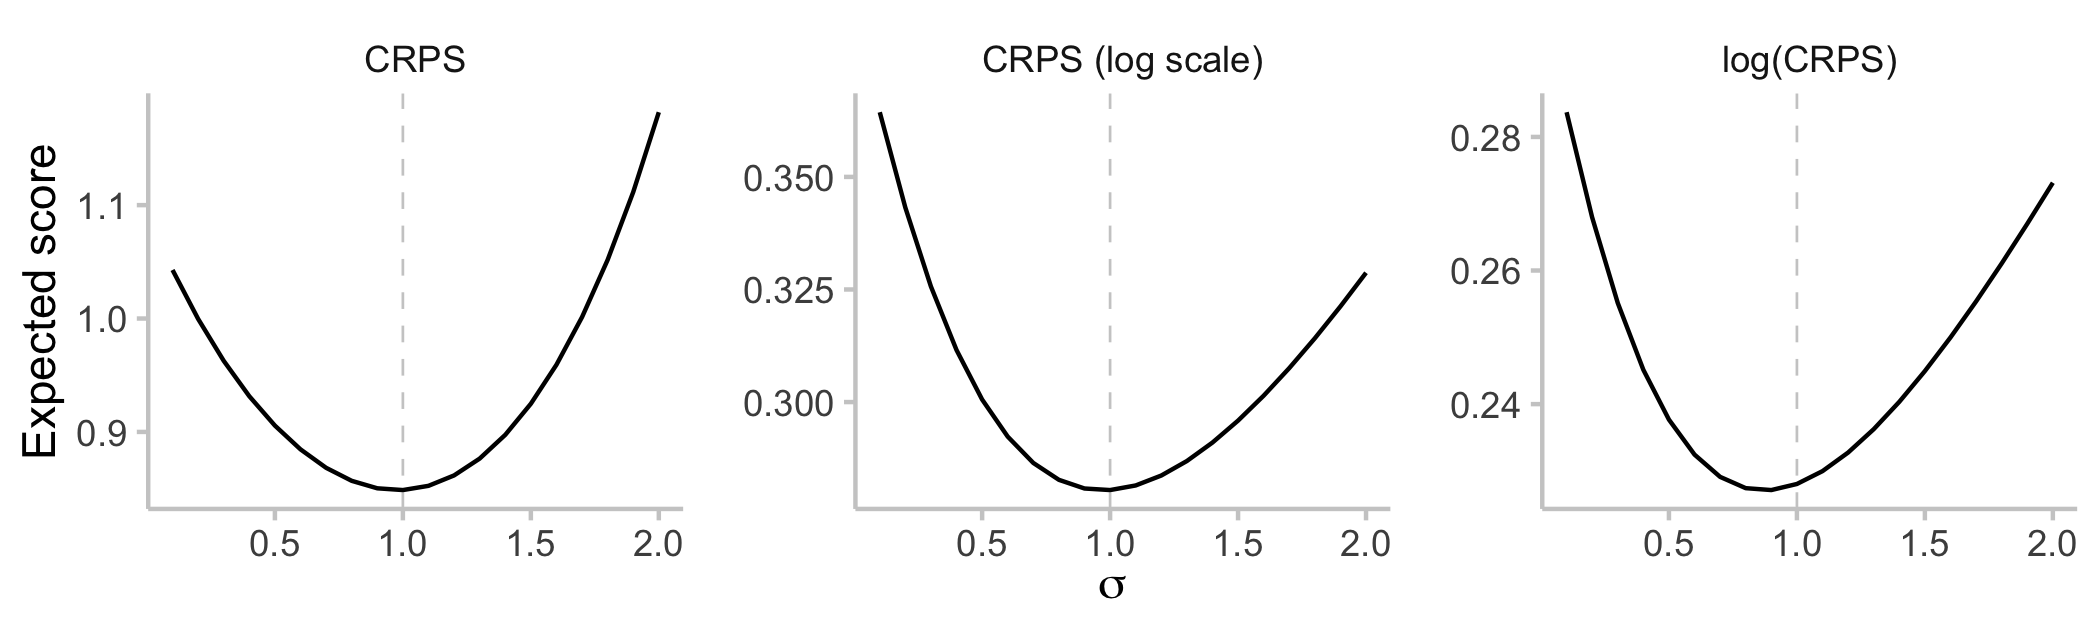
\includegraphics[width=0.99\textwidth]{output/figures/example-log-first.png}
    \caption{Illustration of impropriety of log-transformed CRPS. We assume $Y \sim \text{LogNormal}(0, 1)$ and evaluate the expected CRPS for predictive distributions $\text{LogNormal}(0, \sigma)$ with varying values of $\sigma \in [0.1, 2]$. For the regular CRPS (left) and CRPS applied to log-transformed outcomes (middle), the lowest expectation is achieved for the true value $\sigma = 1$. For the log-transformed CRPS, the optimal value is  0.9, i.e. there is an incentive to report a forecast that is too sharp.}
    \label{fig:log-improper}
\end{figure}

In practice, one issue with transformations, such as the log transform, is that they are not readily applicable to negative numbers or zero values, which need to be removed or otherwise handled. 
One common approach to deal with zeros is to add a small quantity, such as 1, to all observations and predictions before taking the logarithm \citep{bellegoDealingLogsZeros2022}. This represents a strictly monotonic transformation and therefore preserves the propriety of the resulting score. The choice of the quantity to add does however influences scores and rankings, as measures of relative errors shrink when adding a constant to the forecast and the observation. The impact is greatest for forecasts of small quantities, as relative errors shrink more the smaller the original value before adding a constant. In principle, it would also be possible to exploit the difference in how scores are affected in order to equalise scores for forecasts of quantities across different scales by adding a larger number (e.g. 100 or 10,000) if average scores are dominated too strongly by forecasts for small quantities. 

Small discrete observed values can pose an additional problem as it may be difficult to reliably evaluate relative errors. A related issues occurs when the predictive distribution has a large probability mass on zero (or on very small values), as this can translate into an excessively wide forecast in relative terms. This can be seen in Figure \ref{fig:HUB-model-comparison-baseline}, where the dispersion component of the WIS is inflated for scores obtained after applying the natural logarithm where forecasts contained zero in its prediction intervals. 

\subsection{Effects on model rankings}
\label{sec:methods:rankings}
Rankings between different forecasters based on the CRPS may change when making use of a transformation, both in terms of aggregate and individual scores. We illustrate this in Figure \ref{fig:illustration-ranking} with two forecasters, A and B, issuing two different distributions with different dispersion. When showing the obtained CRPS as a function of the observed value, it can be seen that the ranking between the two forecasters may change when scoring the forecast on the logarithmic, rather than the natural scale. In particular, on the natural scale, forecaster A, who issues a more uncertain distribution, receives a better score than forecaster B for observed values far away from the centre of the respective predictive distribution. On the log scale, however, forecaster A receives a lower score for large observed values, being more heavily penalised for assigning large probability to small values (which, in relative terms, are far away from the actual observation). 


\begin{figure}[h!]
\centering
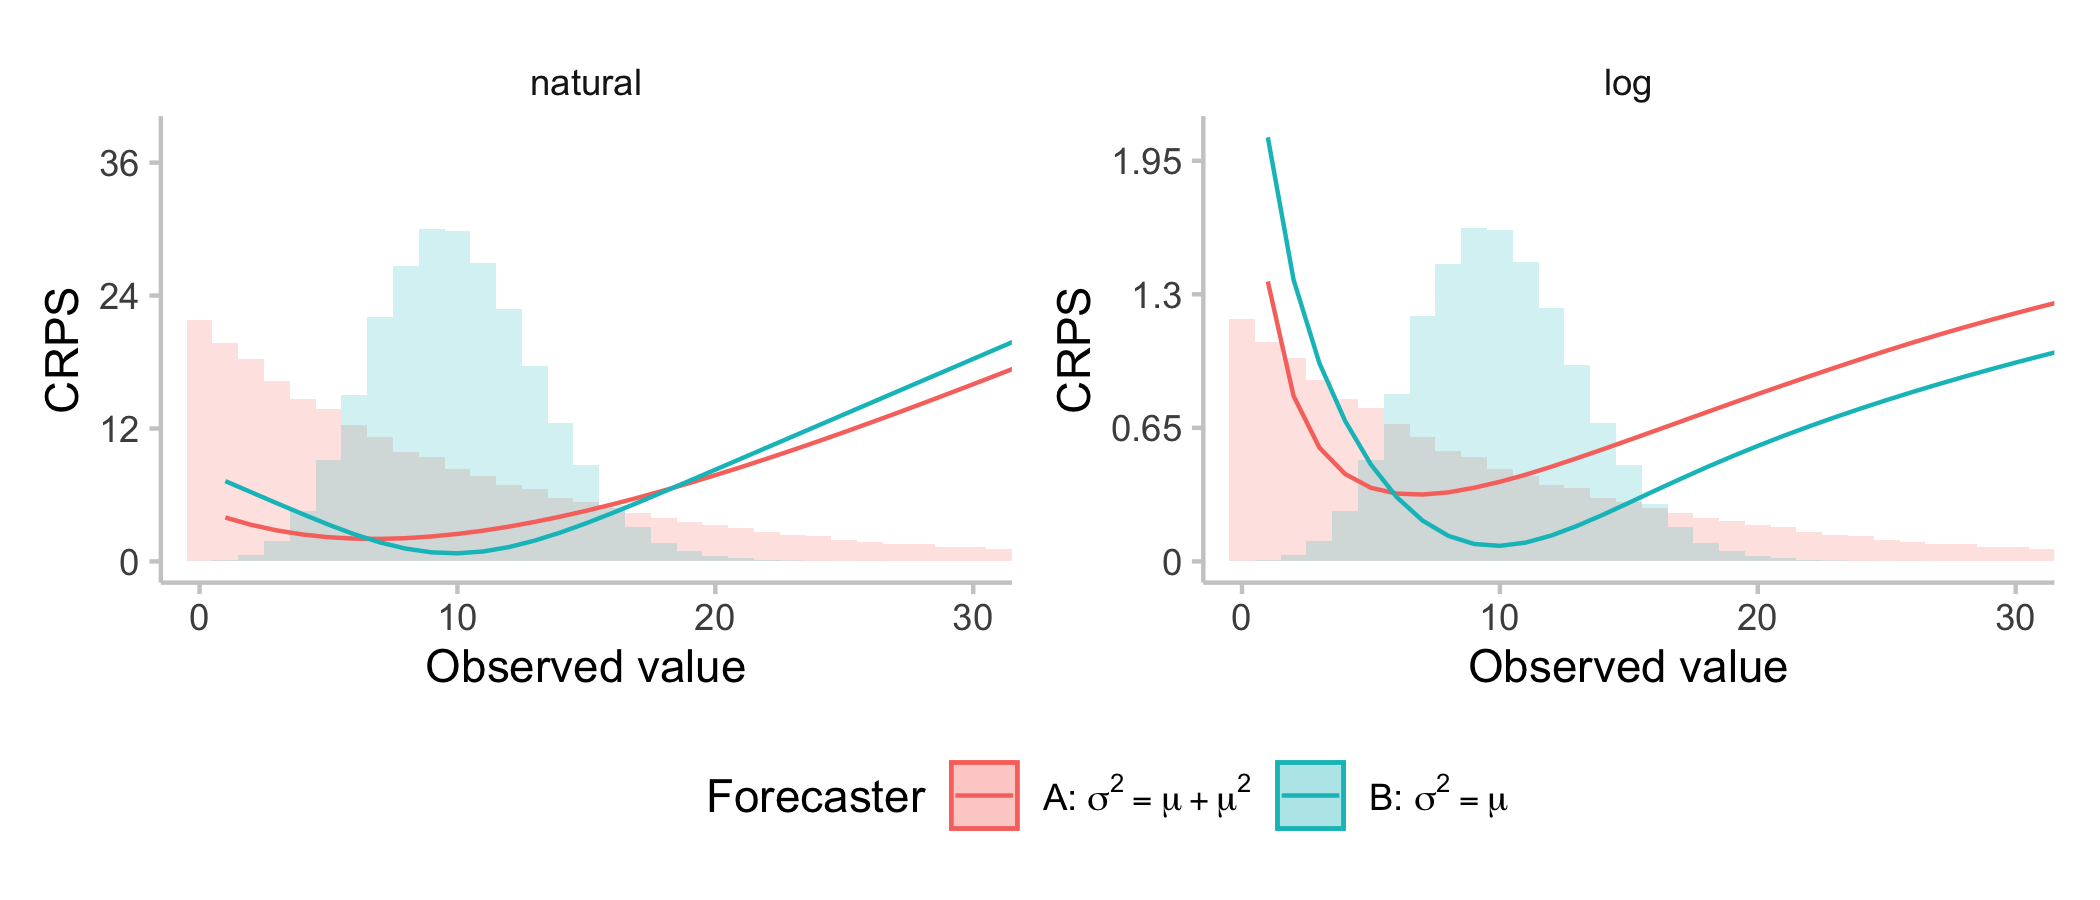
\includegraphics[width = 1\textwidth]{output/figures/illustration-effect-log-ranking-crps.png}
\caption{Illustration of the effect of the log-transformation of the ranking for a single forecast. Shown are CRPS (or WIS, respectively) values as a function of the observed value for two forecasters. Model A issues a geometric distribution with mean $\mu = 10$ and variance $\sigma^2 = \mu + \mu^2 = 110$), while Model B issues a Poisson distribution with mean and variance equal to 10. Zeroes in this illustrative example were handled by adding one before applying the natural logarithm.}
\label{fig:illustration-ranking}
\end{figure}

Overall model rankings would be expected to differ even more when scores are averaged across multiple forecasts or targets. The change in rankings of aggregate scores is mainly driven by the order of magnitude of scores for different forecast targets across time, location and target type and less so by the kind of changes in model rankings for single forecasts discussed above. Large observations will dominate average CRPS values when evaluation is done on the natural scale, but much less so after log transformation. Depending on the relationship between the mean and variance of the forecast target, a log-transformation may even lead to systematically larger scores assigned to small forecast targets, as illustrated in Figure \ref{fig:SIM-wis-state-size-mean}. 

%A different transformation like the square-root may then be more appropriate to make scores independent of the mean of the target quantity (as discussed in Section \ref{sec:methods:vst}). 

%Whether forecasts of small or large targets receive higher scores than those for targets with larger quantities, depends on the relationship between the mean and the variability of the quantity of interest (see Section \ref{sec:methods:vst}. For the simulated count data, log predictions for small quantities received on average higher scores than forecasts for large quantities if the mean and the variance grew at the same rate $\sigma^2 = \mu$, about equal scores when the variance grew at a rate of $\sigma^2 = \mu + \mu^2$ (which for large $\mu$ is dominated by the quadratic term), and smaller scores when the variance grew faster than that (Figure \ref{fig:SIM-wis-state-size-mean}). 

\section{Empirical example: the European Forecast Hub}
\label{sec:results}

\subsection{Setting}

As an empirical comparison of evaluating forecasts on the natural and on the log scale, we use forecasts from the European Forecast Hub \citep{europeancovid-19forecasthubEuropeanCovid19Forecast2021, sherrattPredictivePerformanceMultimodel2022}. 
The European COVID-19 Forecast Hub is one of several COVID-19 Forecast Hubs \citep{cramerEvaluationIndividualEnsemble2021, bracherShorttermForecastingCOVID192021} which have been systematically collecting, aggregating and evaluating forecasts of several COVID-19 targets created by different teams every week. Forecasts are made one to four weeks ahead into the future and follow a quantile-based format with a set of 23 quantiles ($0.01, 0.025, 0.05, ..., 0.5, ... 0.95, 0.975, 0.99$). 

The forecasts used for the purpose of this illustration are forecasts submitted between the 8th of March 2021 and the 12th of May 2022 \textbf{CHECK AGAIN} for reported cases and deaths from COVID-19. We filtered all forecasts submitted to the Hub to only include models which have submitted forecasts for both deaths and cases for 4 horizons in 32 locations on at least 16 CHECK AGAIN forecast dates (see Figure \ref{fig:HUB-num-avail-models}). We removed all observations marked as data anomalies by the European Forecast Hub \citep{sherrattPredictivePerformanceMultimodel2022} as well as all remaining negative observed values. In addition, we filtered out erroneous forecasts characterised by a median forecast of 0 and an actual observed value of larger than 150. All predictive quantiles were truncated at 0. We applied the log-transformation after adding 1 to all predictions and observed values. Where not otherwise stated, we report results for a two-week-ahead forecast horizon. 

In addition to the WIS we use pairwise comparisons \citep{cramerEvaluationIndividualEnsemble2021} to evaluate the relative performance of models across countries in the presence of missing forecasts. In the first step, score ratios are computed for all pairs of models by taking the set of overlapping forecasts between the two models and dividing the score of one model by the score achieved by the other model. The relative skill for a given model compared to others is then obtained by taking the geometric mean of all score ratios which involve that model. Low values are better, and the average model receives a relative skill score of 1. 

\subsection{Illustration and qualitative observations}

Show and discuss Fig 7 here? CHECK AGAIN

\subsection{Descriptive analysis of observed values and scores obtained on the natural and logarithmic scales CHECK AGAIN} 

\begin{figure}[h!]
    \centering
    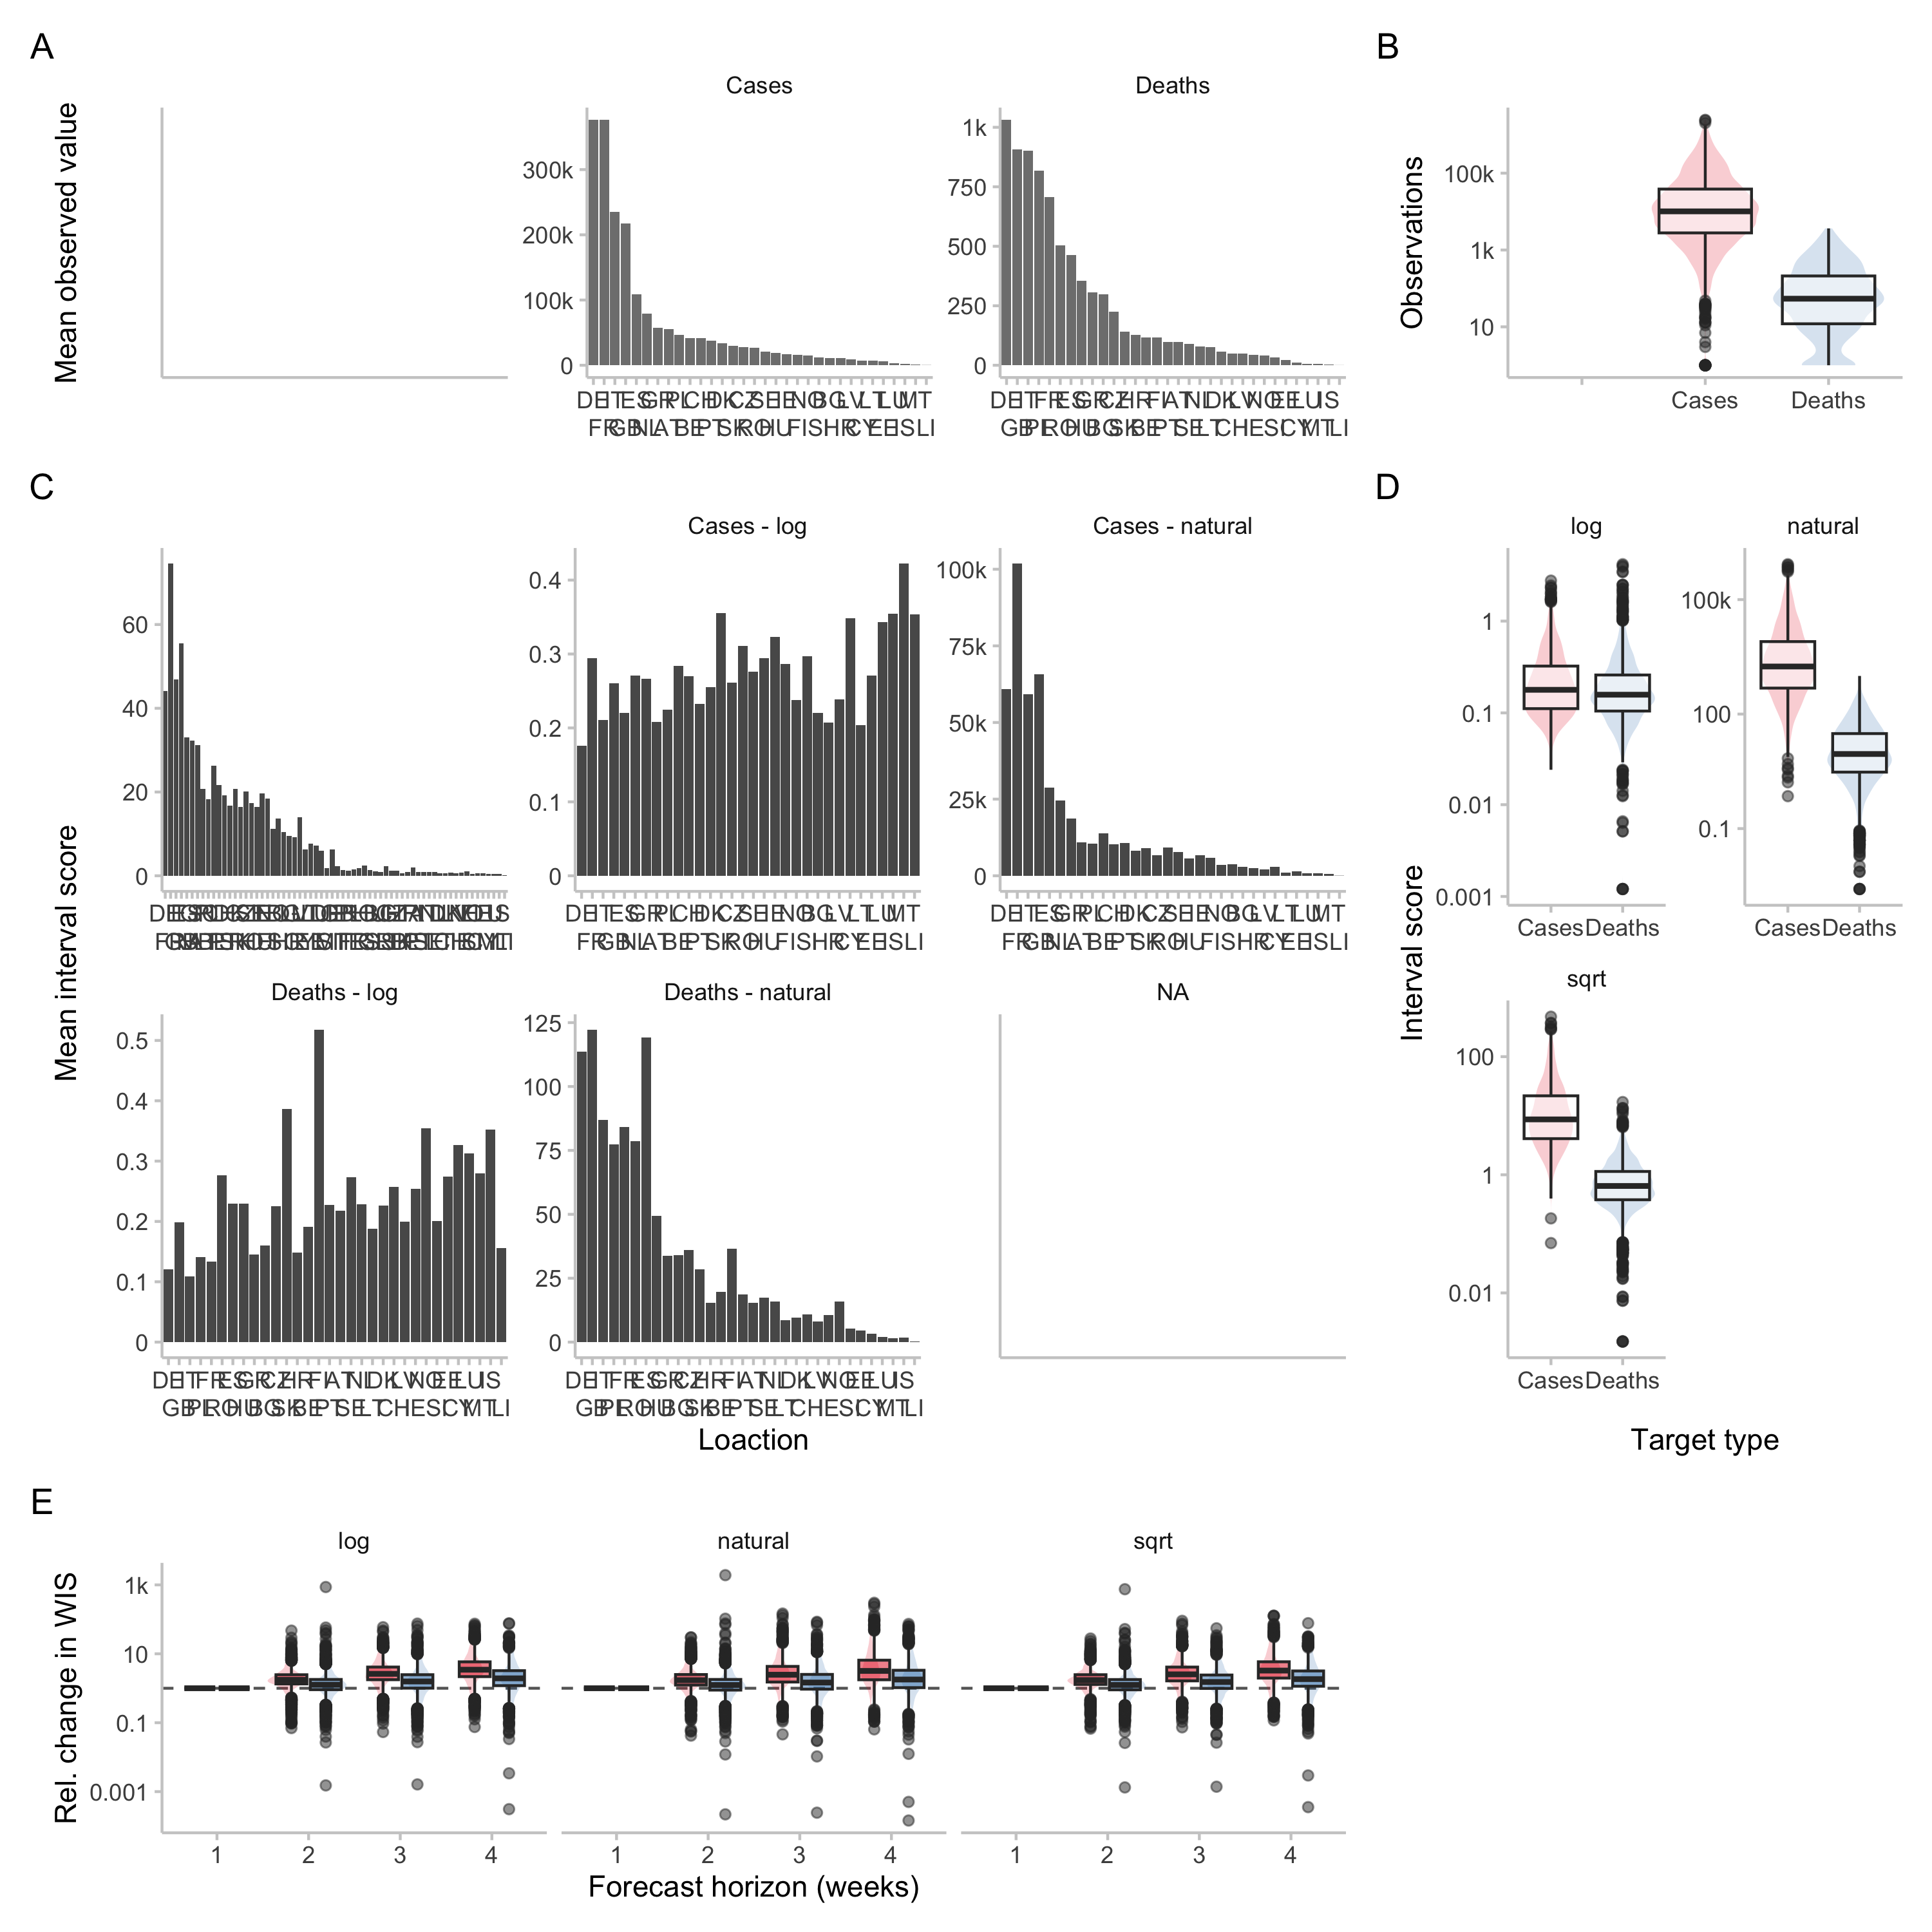
\includegraphics[width=0.99\textwidth]{output/figures/HUB-mean-obs-location.png}
    \caption{Observations and scores across locations and forecast horizons for the European COVID-19 Forecast Hub data. Locations are sorted according to the mean observed value in that location. 
    A: Average (across all time points) of observed cases and deaths for different locations. B: Corresponding boxplot (y-axis on log-scale) of all cases and deaths. C: Scores for two-week-ahead forecasts from the EuroCOVIDhub-ensemble (averaged across all forecast dates) for different locations, evaluated on the natural as well as the logarithmic scale. D: Corresponding boxplots of all individual scores for two-week-ahead predictions. E: Boxplots for the relative change of scores for the EuroCOVIDhub-ensemble across forecast horizons. For any given forecast date and location, forecasts were made for four different forecast horizons, resulting in four scores. All scores were divided by the score for forecast horizon one.}
    \label{fig:HUB-mean-locations}
\end{figure}

Across the dataset, the average number of observed cases and deaths varied considerably by location and target type (see Figure \ref{fig:HUB-mean-locations}A and B). On the natural scale, scores also varied considerably across targets (see Figure\ref{fig:HUB-mean-locations}D) and locations (see Figure\ref{fig:HUB-mean-locations}C). On the log scale, scores were more evenly distributed between targets (see Figure\ref{fig:HUB-mean-locations}D) and locations (see Figure\ref{fig:HUB-mean-locations}C). Both on the natural scale as well to a slightly lesser extent on the log scale, scores increased considerably with increasing forecast horizon (see Figure \ref{fig:HUB-mean-locations}E). This reflects the increasing difficulty of forecasts further into the future and, for the log scale, corresponds with our expectations from Section \ref{sec:methods:growthrate}. 

\begin{figure}[h!]
    \centering
    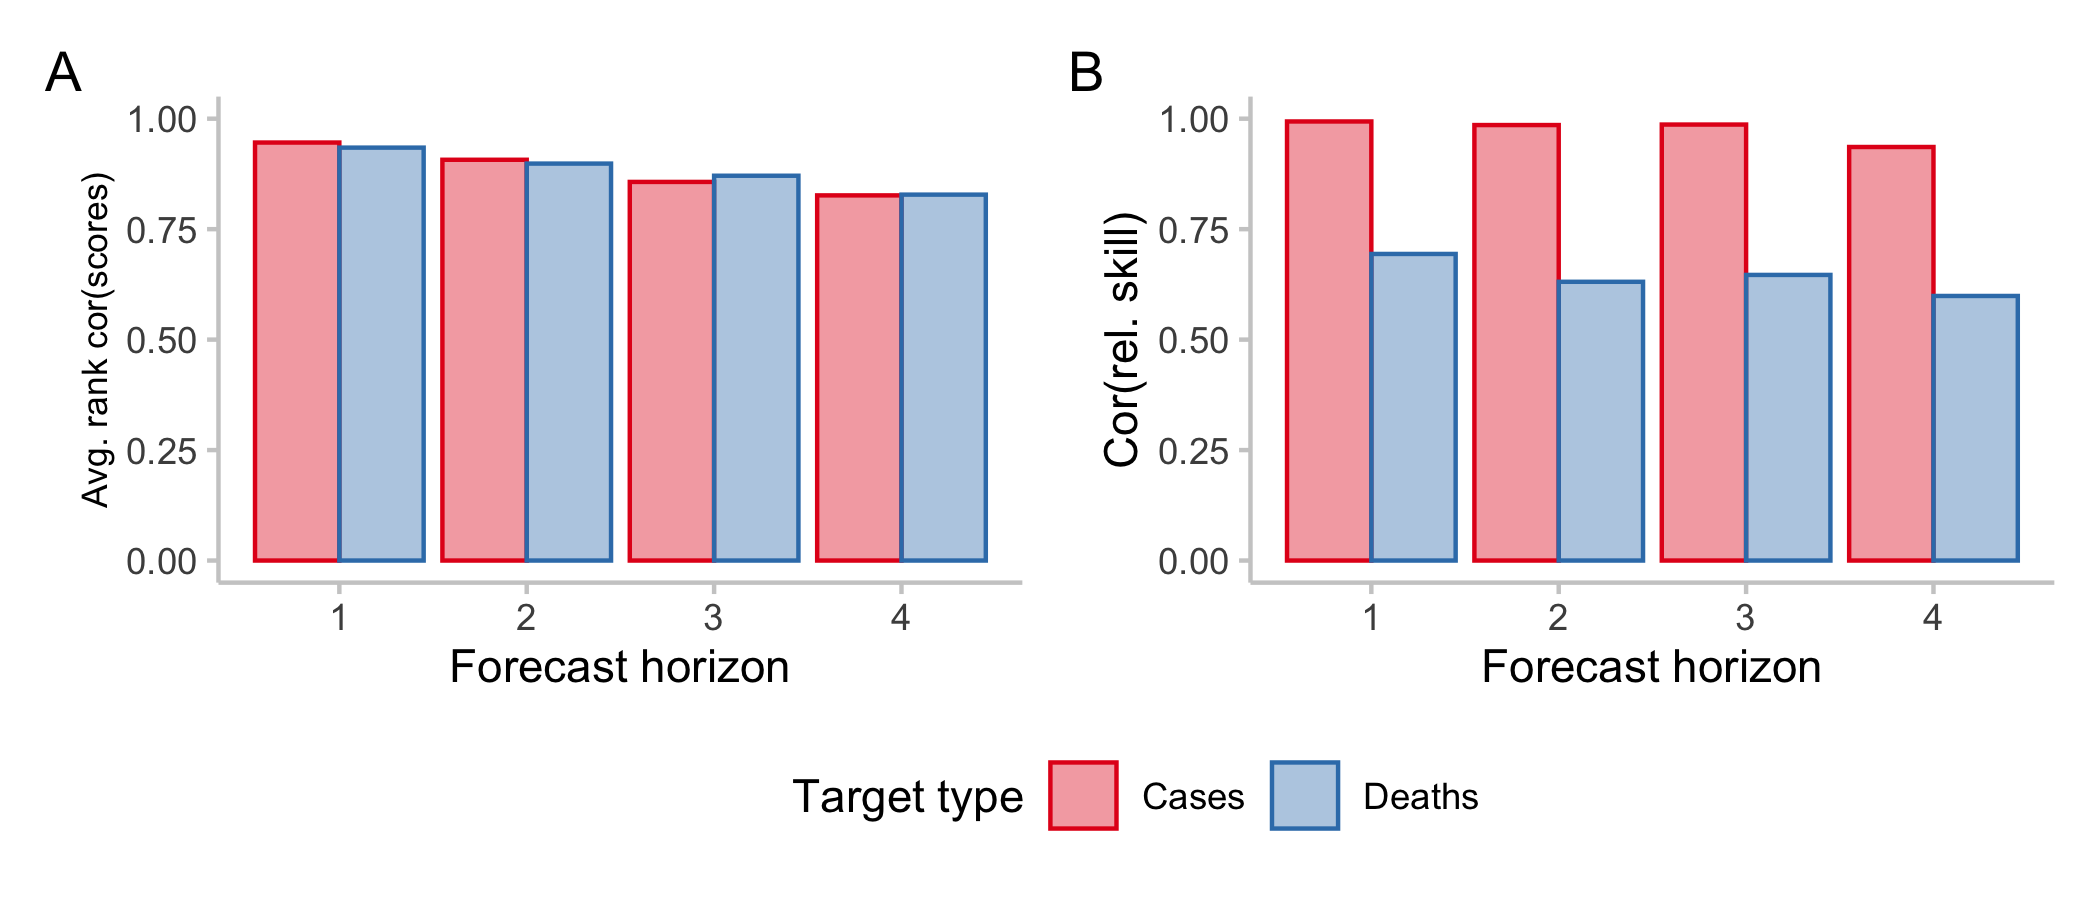
\includegraphics[width=0.99\textwidth]{output/figures/HUB-correlations.png}
    \caption{Correlations for median forecasts, scores, and rankings on the natural and logarithmic scale. A: WIS for two-week-ahead predictions of the EuroCOVIDhub-ensemble against median predicted values. B: Average Spearman rank correlation of scores for individual forecasts from all models. For every individual target (defined by a combination of forecast date, target type, horizon, location), one score was obtained per model. Then, the rank correlation was computed between the scores for all models on the natural scale vs. on the log scale. All rank correlations were averaged across locations, and target types and stratified by horizon and target type. C: Correlation between relative skill scores. For every forecast horizon and target type, a separate rel. skill score was computed per model using pairwise comparisons. The plot shows the correlation between the rel. skill scores on the natural vs. on the log scale.}
    \label{fig:HUB-cors}
\end{figure}

\subsection{Regression analysis to determine the variance-stabilizing transformation}

As argued in Section \ref{sec:methods:vst}, the mean-variance, or mean-CRPS, relationship determines which transformation can serve as a VST. To assess this empirically, we ran the regression

\begin{equation*}
    \log[\text{CRPS}(F, y)] = \alpha + \beta \times \log[\text{median}(F)], 
\end{equation*}
where the predictive distribution $F$ and the observation $y$ are on the natural scale. This is equivalent to
\begin{equation*}
    \text{CRPS}(F, y) = \exp(\alpha) \times \text{median}(F)^\beta, 
\end{equation*}
meaning that we estimate a polynomial relationship between the predictive median and achieved CRPS. Note that we are using predictive medians rather than means as only the former are available in the European COVID-19 Forecast Hub. We applied the regression to case and death forecasts, pooled across horizons and stratified for one through four-week-ahead forecasts. Results are provided in Table \ref{tab:HUB-regression}. It can be seen that the estimates of $\beta$ always take a value below 1.  As the CRPS scales with the standard deviation (see Section \ref{sec:methods:vst}), this can be interpreted as a slightly sub-quadratic mean-variance relationship. The logarithmic transformation should thus approximately stabilize the variance (and CRPS), possibly leading to somewhat higher scores for smaller forecast targets. The square-root transformation, on the other hand, can be expected to still lead to higher CRPS values for targets of higher orders of magnitude.

To check this, we ran the regressions
\begin{equation*}
    \text{CRPS}(F_{\log}, \log y) = \alpha_{\log} + \beta_{\log} \cdot \log{(\text{median}(F))},
\end{equation*}
where $F_{\log}$ is the predictive distribution for $\log(y)$, and
\begin{equation*}
    \text{CRPS}(F_{\sqrt{\ }}, \sqrt{y}) = \alpha_{\sqrt{\ }} + \beta_{\sqrt{\ }} \cdot \sqrt{\text{median}(F)},
\end{equation*} 
where $F_{\sqrt{\ }}$ is the predictive distribution on the square-root scale. As can be seen from Table \ref{tab:HUB-regression}, the results indeed indicate small targets lead to larger average CRPS when using the log transform ($\beta_{\log} < 0$), while the opposite is true for the square-root transform ($\beta_{\sqrt{\ }} > 0$). The results of the three regressions are also displayed in Figure \ref{fig:HUB-cors}. It appears that the log transformation is most suitable to stabilise the CRPS values in this empirical example. 

% We found that on the natural scale, the order of magnitude of the forecast (represented by the median, rather than the mean, as forecasts were stored as quantiles and the mean was not available) strongly influenced scores, with estimated $\beta$-values close to one. On the log scale, this influence was small, with estimated $\beta^*$-values close to zero. Both on the natural and on the log scale we found scores to increase over time (estimated $\alpha$- and $\alpha^*$-values increased over horizons). Estimates are summarised in Table \ref{tab:HUB-regression}. 

\begin{figure}[h!]
    \centering
    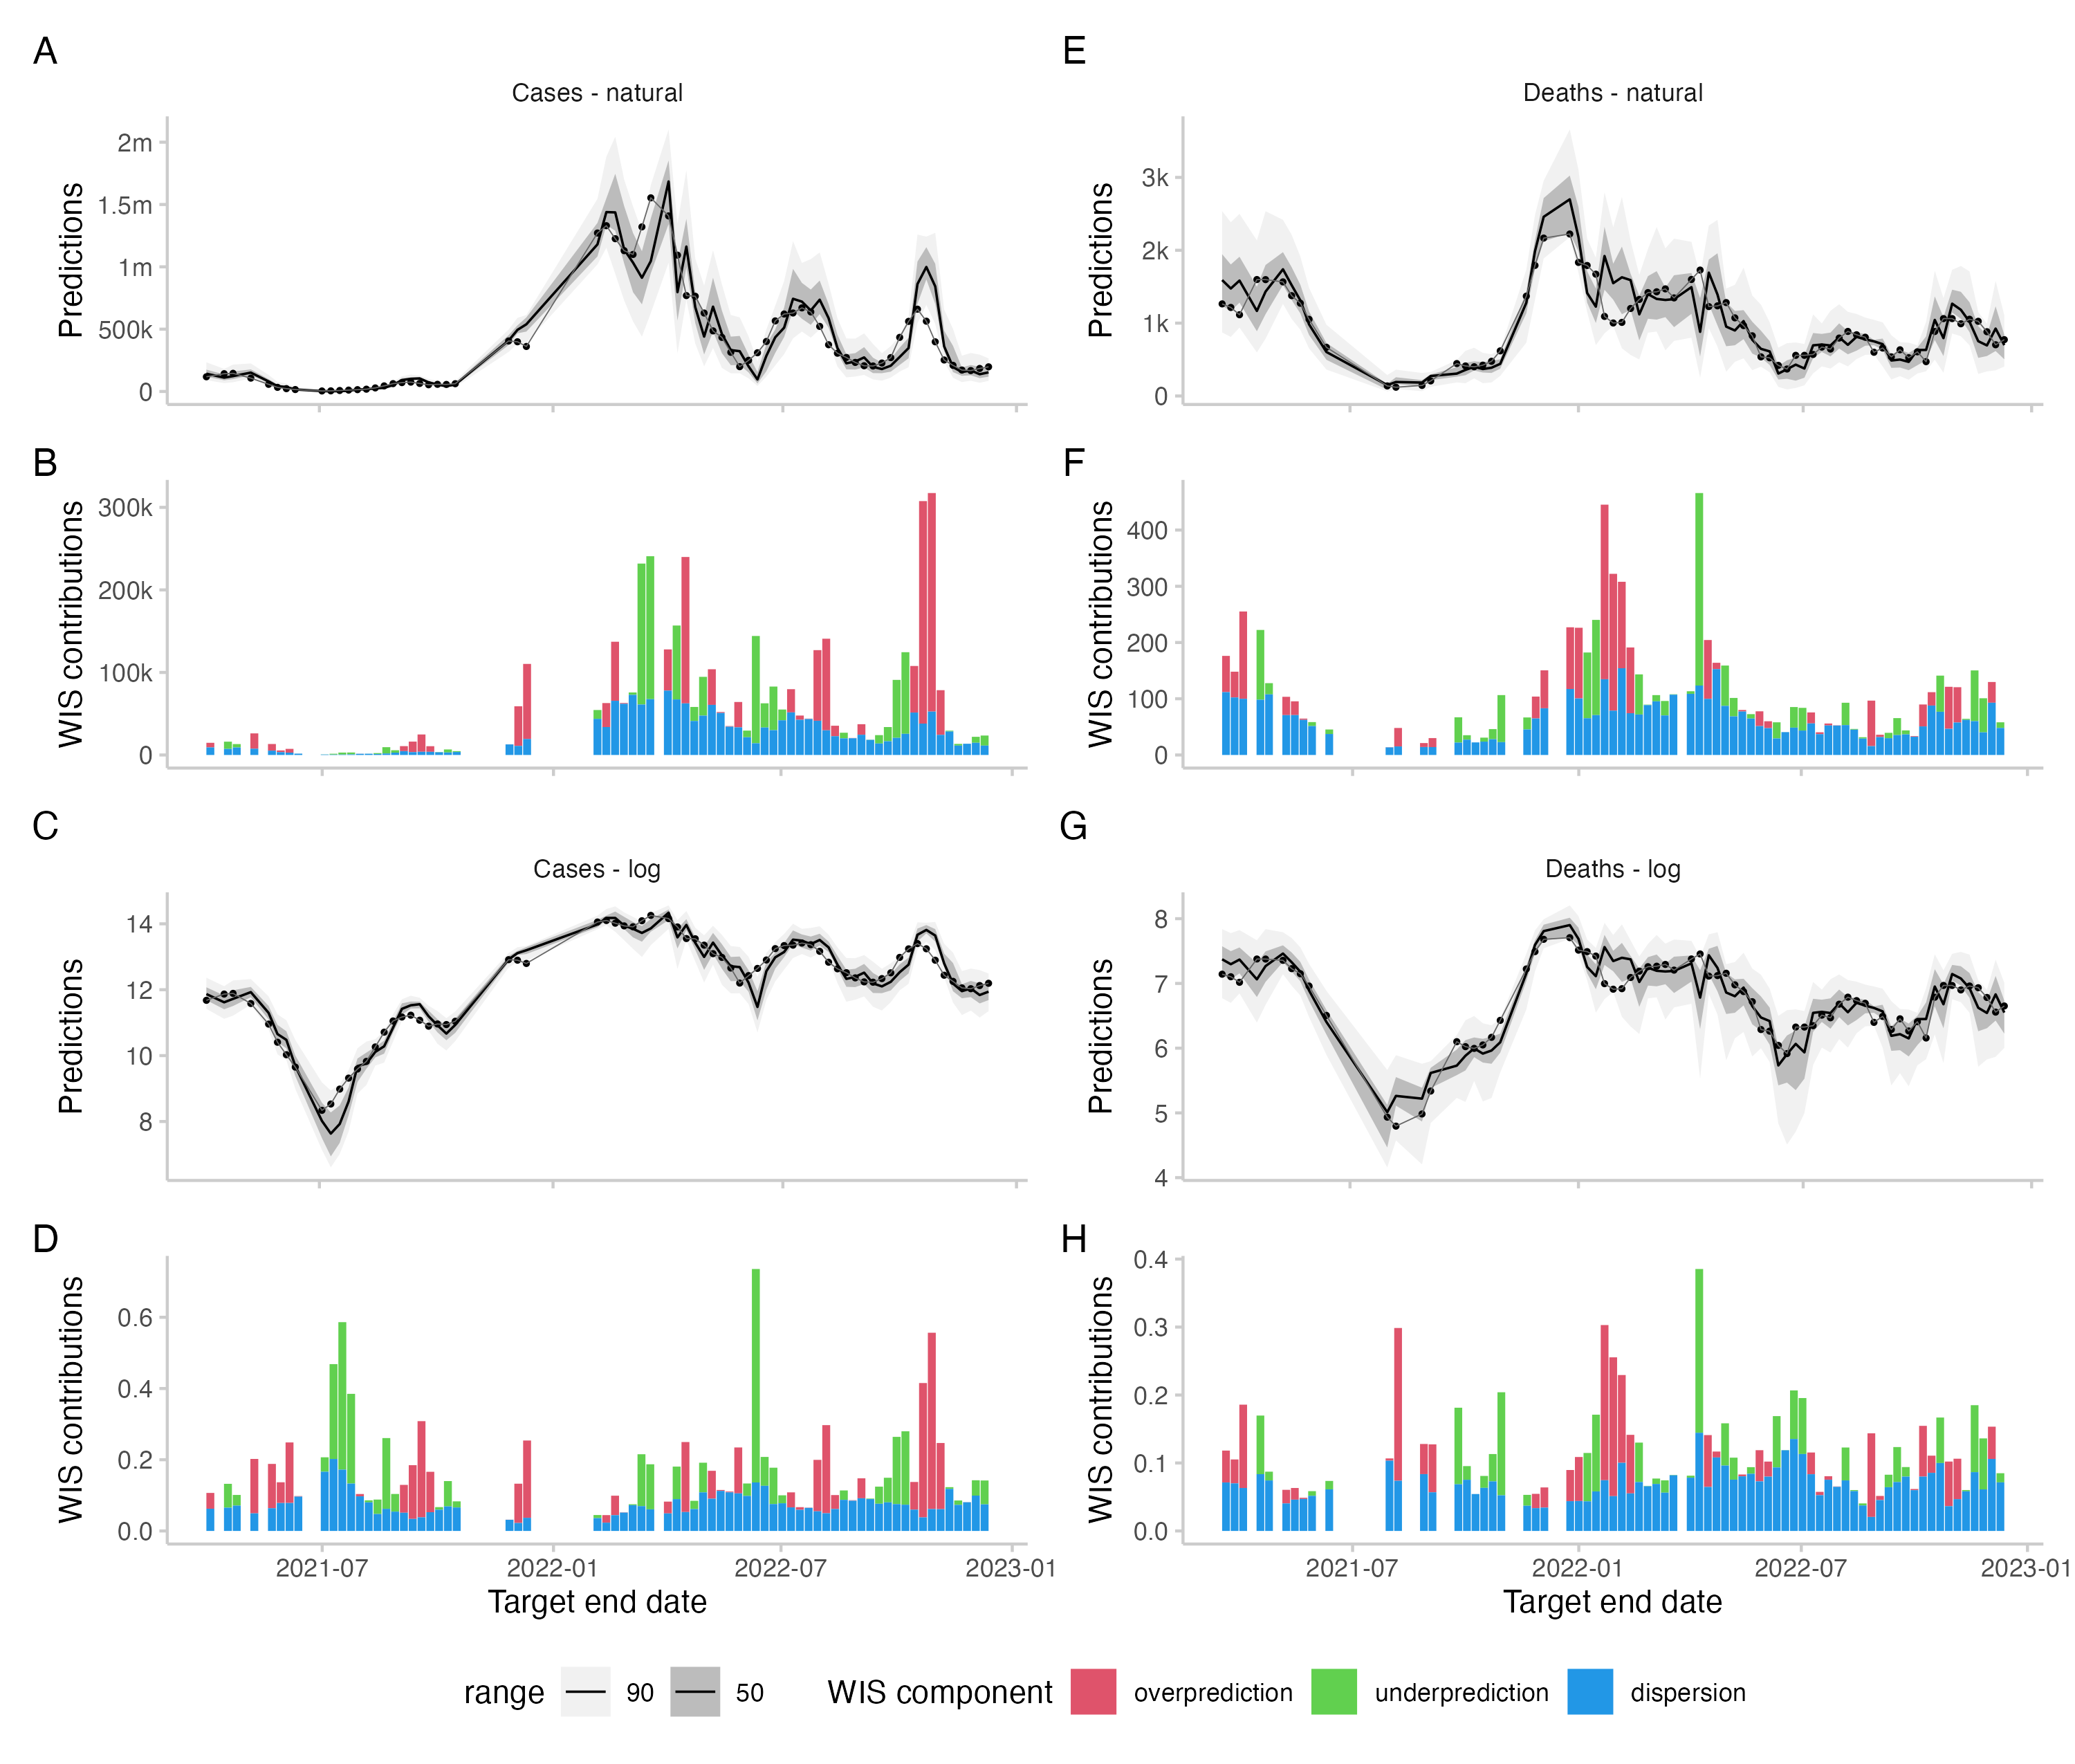
\includegraphics[width=0.99\textwidth]{output/figures/HUB-model-comparison-ensemble.png}
    \caption{
    Forecasts and scores for two-week-ahead predictions from the EuroCOVIDhub-ensemble made in Germany. A, E: 50\% and 90\% prediction intervals and observed values for cases and deaths on the natural scale. B, F: Corresponding scores. C, G: Forecasts and observations on the log scale. D, H: Corresponding scores. 
    }
    \label{fig:HUB-model-comparison-ensemble}
\end{figure}

\subsection{Impact of logarithmic transformation on model rankings}

For \textit{individual} forecasts, rankings between models for single forecasts are mostly preserved, with differences increasing across forecast horizons (see Figure \ref{fig:HUB-cors}B). When evaluating performance \textit{averaged across} different forecasts and forecast targets, relative skill scores of the models change considerably. The change is stronger for cases than for deaths (Figure \ref{fig:HUB-cors}C) and possibly tends to increase with increasing forecast horizon. 

When comparing examples of forecasts on the natural scale with those on the log scale (see Figures \ref{fig:HUB-model-comparison-ensemble}, \ref{fig:HUB-model-comparison-baseline}, \ref{fig:HUB-model-comparison-epinow}) a few interesting patterns emerge. Missing the peak, i.e. predicting increasing numbers while actual observations are already falling, tends to contribute a lot to overall scores on the natural scale (see forecasts in May in Figure \ref{fig:HUB-model-comparison-ensemble}A, B). On the log scale, these have less of an influence, as errors are smaller in relative terms (see \ref{fig:HUB-model-comparison-ensemble}C, D). We hypothesise that the lower correlation between skill scores for cases (compared to the correlation of scores for deaths) as displayed in Figure \ref{fig:HUB-cors}C is related to the fact that outlier forecasts missing the peak are more common for cases than for deaths, and therefore relative skill scores are more strongly affected for cases. 
Conversely, failure to predict an upswing while numbers are still low, is less severely punished on the natural scale (see forecasts in July in Figure \ref{fig:HUB-model-comparison-ensemble} A, B), as overall absolute errors are low. On the log scale, missing lower inflection points tends to lead to more severe penalties (see Figure \ref{fig:HUB-model-comparison-ensemble}C, D)). One can also observe that on the natural scale, scores tend to track the overall level of the target quantity (compare for example forecasts for March-July with forecasts for September-October in Figure \ref{fig:HUB-model-comparison-ensemble}E, F). On the log scale, scores do not exhibit this behaviour and rather increase whenever forecasts are far away from the truth in relative terms, regardless of the overall level of observations. 

\begin{figure}[h!]
    \centering
    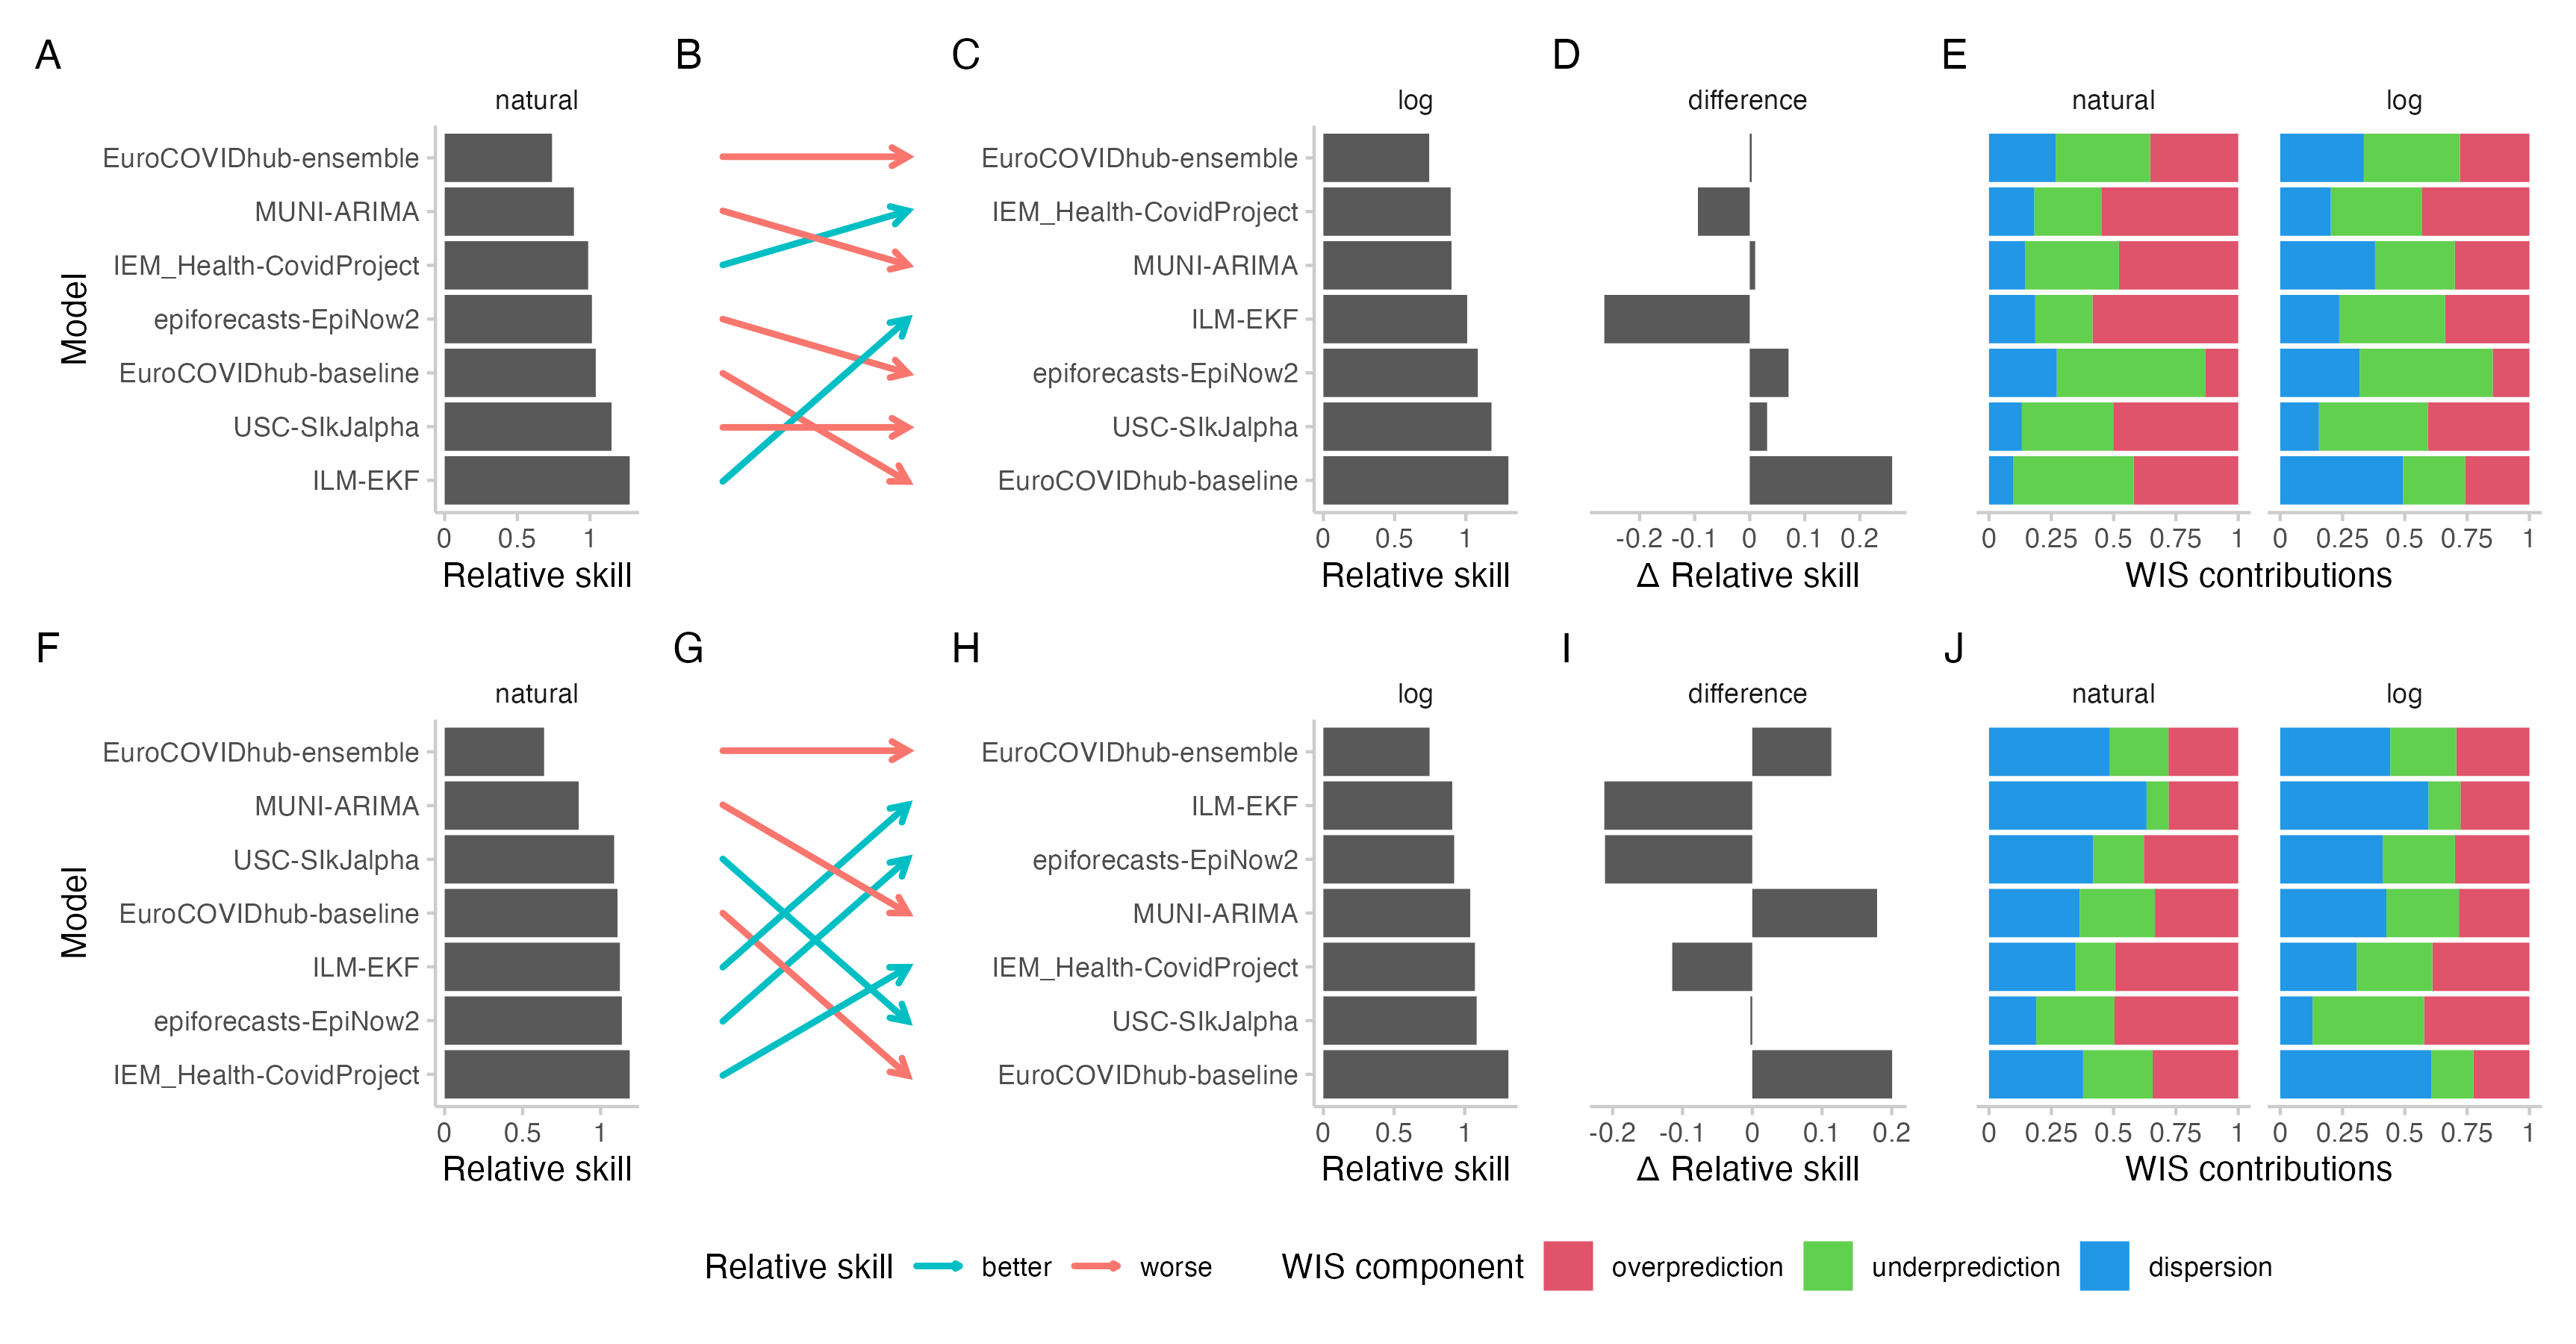
\includegraphics[width=0.99\textwidth]{output/figures/HUB-pairwise-comparisons.png}
    \caption{Changes in model ratings as measured by relative skill for two-week-ahead predictions for cases (top row) and deaths (bottom row). A: Relative skill scores for case forecasts from different models submitted to the European COVID-19 Forecast Hub computed on the natural scale. B: Change in rankings as determined by relative skill scores when moving from an evaluation on the natural scale to one on the logarithmic scale. C: Relative skill scores based on scores on the log scale. D: Difference in relative skill scores computed on the natural and on the logarithmic scale. E: Relative contributions of the different WIS components (overprediction, underprediction, and dispersion) to overall model scores on the natural and the logarithmic scale. F, G, H, I, J, K: Analogously for deaths.}
    \label{fig:HUB-rank-order}
\end{figure}


The rank order of different forecasting models changes noticeably (see Figure \ref{fig:HUB-rank-order}. 
% I removed this part as it doesn't seem accurate anymore / we don't even have all the models in there anymore. 
%indicates that models that do not make use of a exponential error model and thus would be biased towards under-prediction during periods of exponential growth, such as the MUNI-ARMA model, were ranked lower when using a log-transform. The epiforecasts-EpiNow2 forecast model, on the other hand~(created by co-authors of this study), which makes forecasts based on the behaviour of the reproduction number and thus implicitly uses an exponential error model, was the most impacted by the change to log-scale scoring moving from last place for reported cases to 4th place. Other models that are based on modelling the growth rate, such as the LANL-GrowthRate forecaster, do less well after a log-transform, indicating that this potential association between model structure and score under different approximations does not hold strictly.
Encouragingly for the European Forecast Hub, the Hub ensemble, which is the forecast the organisers suggest forecast consumers make use of, remains one of the top forecasts across scoring schemes and indeed ranks higher for reported cases when a log-transform is used.

\section{Discussion}
\label{sec:discussion}

In this paper, we proposed the use of transformations, with a particular focus on the natural logarithmic transformation, when evaluating forecasts in an epidemiological setting. These transformations can address issues that arise when evaluating epidemiological forecasts based on measures of absolute error and their probabilistic generalisations (i.e CRPS and WIS). We showed that scores obtained after log-transforming both forecasts and observations can be interpreted as a) a measure of relative prediction errors, as well as b) a score for a forecast of the exponential growth rate of the target quantity and c) as variance stabilising transformation in some settings.
When applying this approach to forecasts from the European COVID-19 Forecast Hub, we found overall scores on the log scale to be more equal across, time, location and target type (cases, deaths) than scores on the natural scale. Scores on the log scale were much less influenced by the overall incidence level in a country and showed a slight tendency to be higher in locations with very low incidences. We found that model rankings changed noticeably. 
%, favouring models like epiforecasts-EpiNow2 which uses a log scale generative process and a negative binomial observation model, and disfavouring models like MUNI-ARIMA which uses a square root transform to stabilise variance. 
On the natural scale, missing the peak and overshooting was more severely penalised than missing the nadir and the following upswing in numbers. Both failure modes tended to be more equally penalised on the log scale (with undershooting receiving slightly higher penalties in our example). 

Applying a log-transformation prior to the WIS means that forecasts are evaluated in terms of relative errors and errors on the exponential growth rate, rather than absolute errors. The most important strength of this approach is that the evaluation better accommodates the exponential nature of the epidemiological process and the types of errors forecasters who accurately model those processes are expected to make. The log-transformation also helps avoid issues with scores being strongly influenced by the order of magnitude of the forecast quantity, which can be an issue when evaluating forecasts on the natural scale. 
A potential downside is that forecast evaluation is unreliable in situations where observed values are zero or very small. Including very small values in prediction intervals (see e.g. Figure \ref{fig:HUB-model-comparison-baseline}) can lead to excessive dispersion values on the log scale. 
Similarly, locations with lower incidences may get disproportionate weight (i.e. high scores) when evaluating forecasts on the log scale. \cite{bracherEvaluatingEpidemicForecasts2021} argue that the large weight given to forecasts for locations with high incidences is a desirable property, as it reflects performance on the targets we should care about most. On the other hand, scoring forecasts on the log scale may be less influenced by outliers and better reflect consistent performance across time, space, and forecast targets. It also gives higher weight to another type of situation one may care about, namely one in which numbers start to rise from a previously low level. 
If one is interested in scoring a forecast of the multiplicative, rather than the exponential growth rate, it may be better to use a different transformation, e.g. dividing every forecast and corresponding observed value by the previously last observed value when the forecast was made. 

The log-transformation is only one of many transformations that may be useful and appropriate in an epidemiological context. One obvious option is to apply a population standardization to obtain incidence forecasts e.g., per 100,000 population If one is interested in multiplicative, rather than exponential growth rates, one could convert forecasts into forecasts for the multiplicative growth rate by dividing numbers by the last observed value. We suggested using the natural logarithm as a variance-stabilising transformation (VST) or alternatively the square-root transformation in the case of a Poisson distributed variable. Other VST like the Box-Cox \citep{boxAnalysisTransformations1964} are conceivable as well. Another promising transformation would be to take differences between forecasts on the log scale, or alternatively to divide each forecast by the forecast of the previous week (and analogously for observations), in order to obtain forecasts for week-to-week growth rates. One could then also ask forecasters to provide estimates of the weekly relative change applied to the latest data and subsequent forecast points directly. This would be akin to evaluating the shape of the predicted trajectory against the shape of the observed trajectory \citep[for a different approach to evaluating the shape of a forecast, see][]{srivastavaShapebasedEvaluationEpidemic2022}. This, unfortunately, is not feasible for forecasts stored as predictive quantiles, as the growth rate of the $\alpha$-quantile may be different from the $\alpha$-quantile of the growth-rate, but may be an interesting approach if predictive samples are available. It is possible to go beyond choosing a single transformation by constructing composite scores as a weighted sum of scores based on different transformations. This would make it possible to create custom scores and allow forecast consumers to assign explicit weights to different qualities of the forecasts they might care about.

In this work, we focused on the CRPS and WIS, which are widely used in the evaluation of epidemic forecasts. We note that for the logarithmic score, which has also been used e.g., in some editions of the FluSight challenge \cite{reichCollaborativeMultiyearMultimodel2019}, the question of the right scale to evaluate forecasts does not arise. It is known that log score differences between different forecasters are invariant to monotonic transformations of the outcome variable (see e.g., \citealt{Diks2011}). This is clearly an advantage of the logarithmic score over the CRPS; however, the logarithmic score is known to have other severe downsides, e.g., its low robustness to sporadically misguided forecasts; see \cite{bracherEvaluatingEpidemicForecasts2021} for a more detailed discussion.

Exploring transformations is a promising avenue for future work that could help bridge the gap between modellers and policymakers by providing scoring rules that better reflect what forecast consumers care about. Potentially, the variance stabilising time-series forecasting literature may be a useful source of transformations for various forecast settings. We have shown that the natural logarithm transformation can lead to significant changes in the relative rankings of models against each other, with potentially important implications for decision-makers who rely on the knowledge of past performance to make a judgement about which forecasts should inform future decisions. While it is commonly accepted that multiple proper scoring rules should usually be considered when comparing forecasts, we think this should be supplemented by considering different transformations of the data to obtain a richer picture of model performance. More work needs to be done to better understand the effects of applying transformations in different contexts, and how they may impact decision-making. 

\newpage

\appendix
\section{Supplementary information}

\subsection{Alternative Formulation of the WIS}
\label{sec:alternative-wis}

Instead of defining the WIS as an average of scores for individual quantiles, we can define it using an average of scores for symmetric predictive intervals. For a single prediction interval, the interval scoren (IS) is computed as the sum of three penalty components, dispersion (width of the prediction interval), underprediction and overprediction,  
%
\begin{linenomath*}
\begin{align*}
 IS_\alpha(F,y) &= (u-l) + \frac{2}{\alpha} \cdot (l-y) \cdot 1(y \leq l) + \frac{2}{\alpha} \cdot (y-u) \cdot 1(y \geq u) \\
 &= \text{dispersion} + \text{underprediction} + \text{overprediction},    
\end{align*}
\end{linenomath*}
%
where $1()$ is the indicator function, $y$ is the observed value, and $l$ and $u$ are the $\frac{\alpha}{2}$ and $1 - \frac{\alpha}{2}$ quantiles of the predictive distribution, i.e. the lower and upper bound of a single central prediction interval. For a set of $K^*$ prediction intervals and the median $m$, the WIS is computed as a weighted sum, 
\begin{linenomath*}
\begin{equation*}
\text{WIS} = \frac{1}{K^* + 0.5} \cdot \left(w_0 \cdot |y - m| + \sum_{k = 1}^{K^*} w_k \cdot IS_{\alpha_{k}}(F, y)\right),    
\end{equation*} 
\end{linenomath*}
where $w_k$ is a weight for every interval. Usually, $w_k = \frac{\alpha_k}{2}$ and $w_0 = 0.5$. 



\begin{table}[h!]
    \centering


\begin{tabular}{lllcc}
\toprule
target\_type & quantity & measure & natural & log\\
\midrule
Cases & Observations & mean & 62004 & 9.19\\
Cases & Observations & sd & 171723 & 2.10\\
Cases & Observations & var & 29488651564 & 4.42\\
\addlinespace
Deaths & Observations & mean & 223 & 3.90\\
Deaths & Observations & sd & 441 & 1.96\\
Deaths & Observations & var & 194221 & 3.85\\
\addlinespace
\hline
\addlinespace
Cases & WIS & mean & 15840 & 0.27\\
Cases & WIS & sd & 53117 & 0.28\\
\addlinespace
Deaths & WIS & mean & 31 & 0.23\\
Deaths & WIS & sd & 65 & 0.28\\
\bottomrule
\end{tabular}
    \caption{Summary statistics for observations and scores for forecasts from the ECDC data set.}
    \label{tab:HUB-summary}
\end{table}

\begin{figure}[h!]
    \centering
    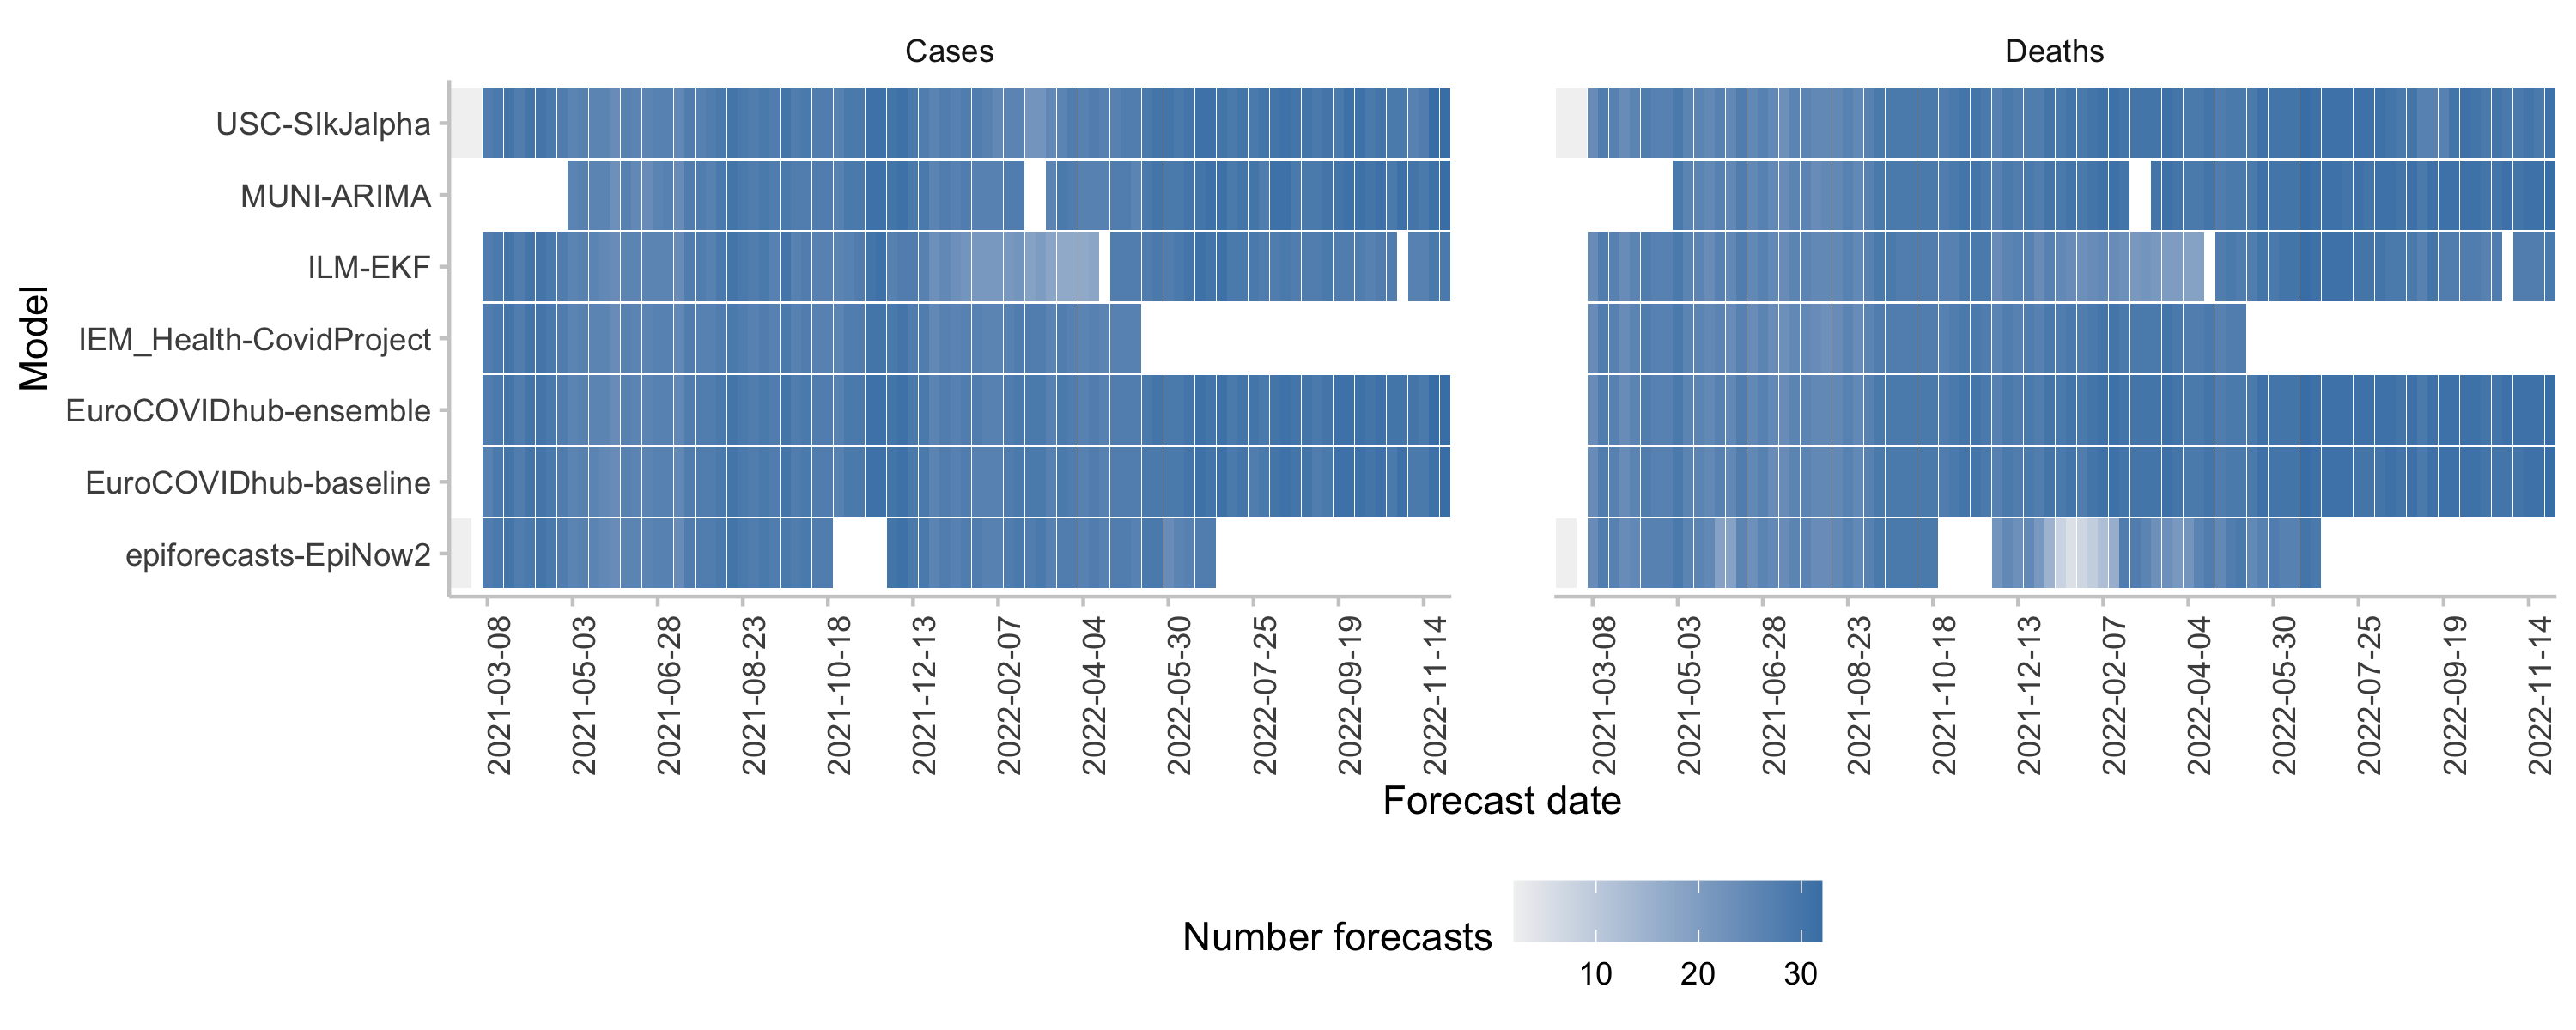
\includegraphics[width=0.99\textwidth]{output/figures/number-avail-forecasts.png}
    \caption{
    Number of forecasts available from different models for each forecast date. 
    }
    \label{fig:HUB-num-avail-models}
\end{figure}


\begin{figure}[h!]
    \centering
    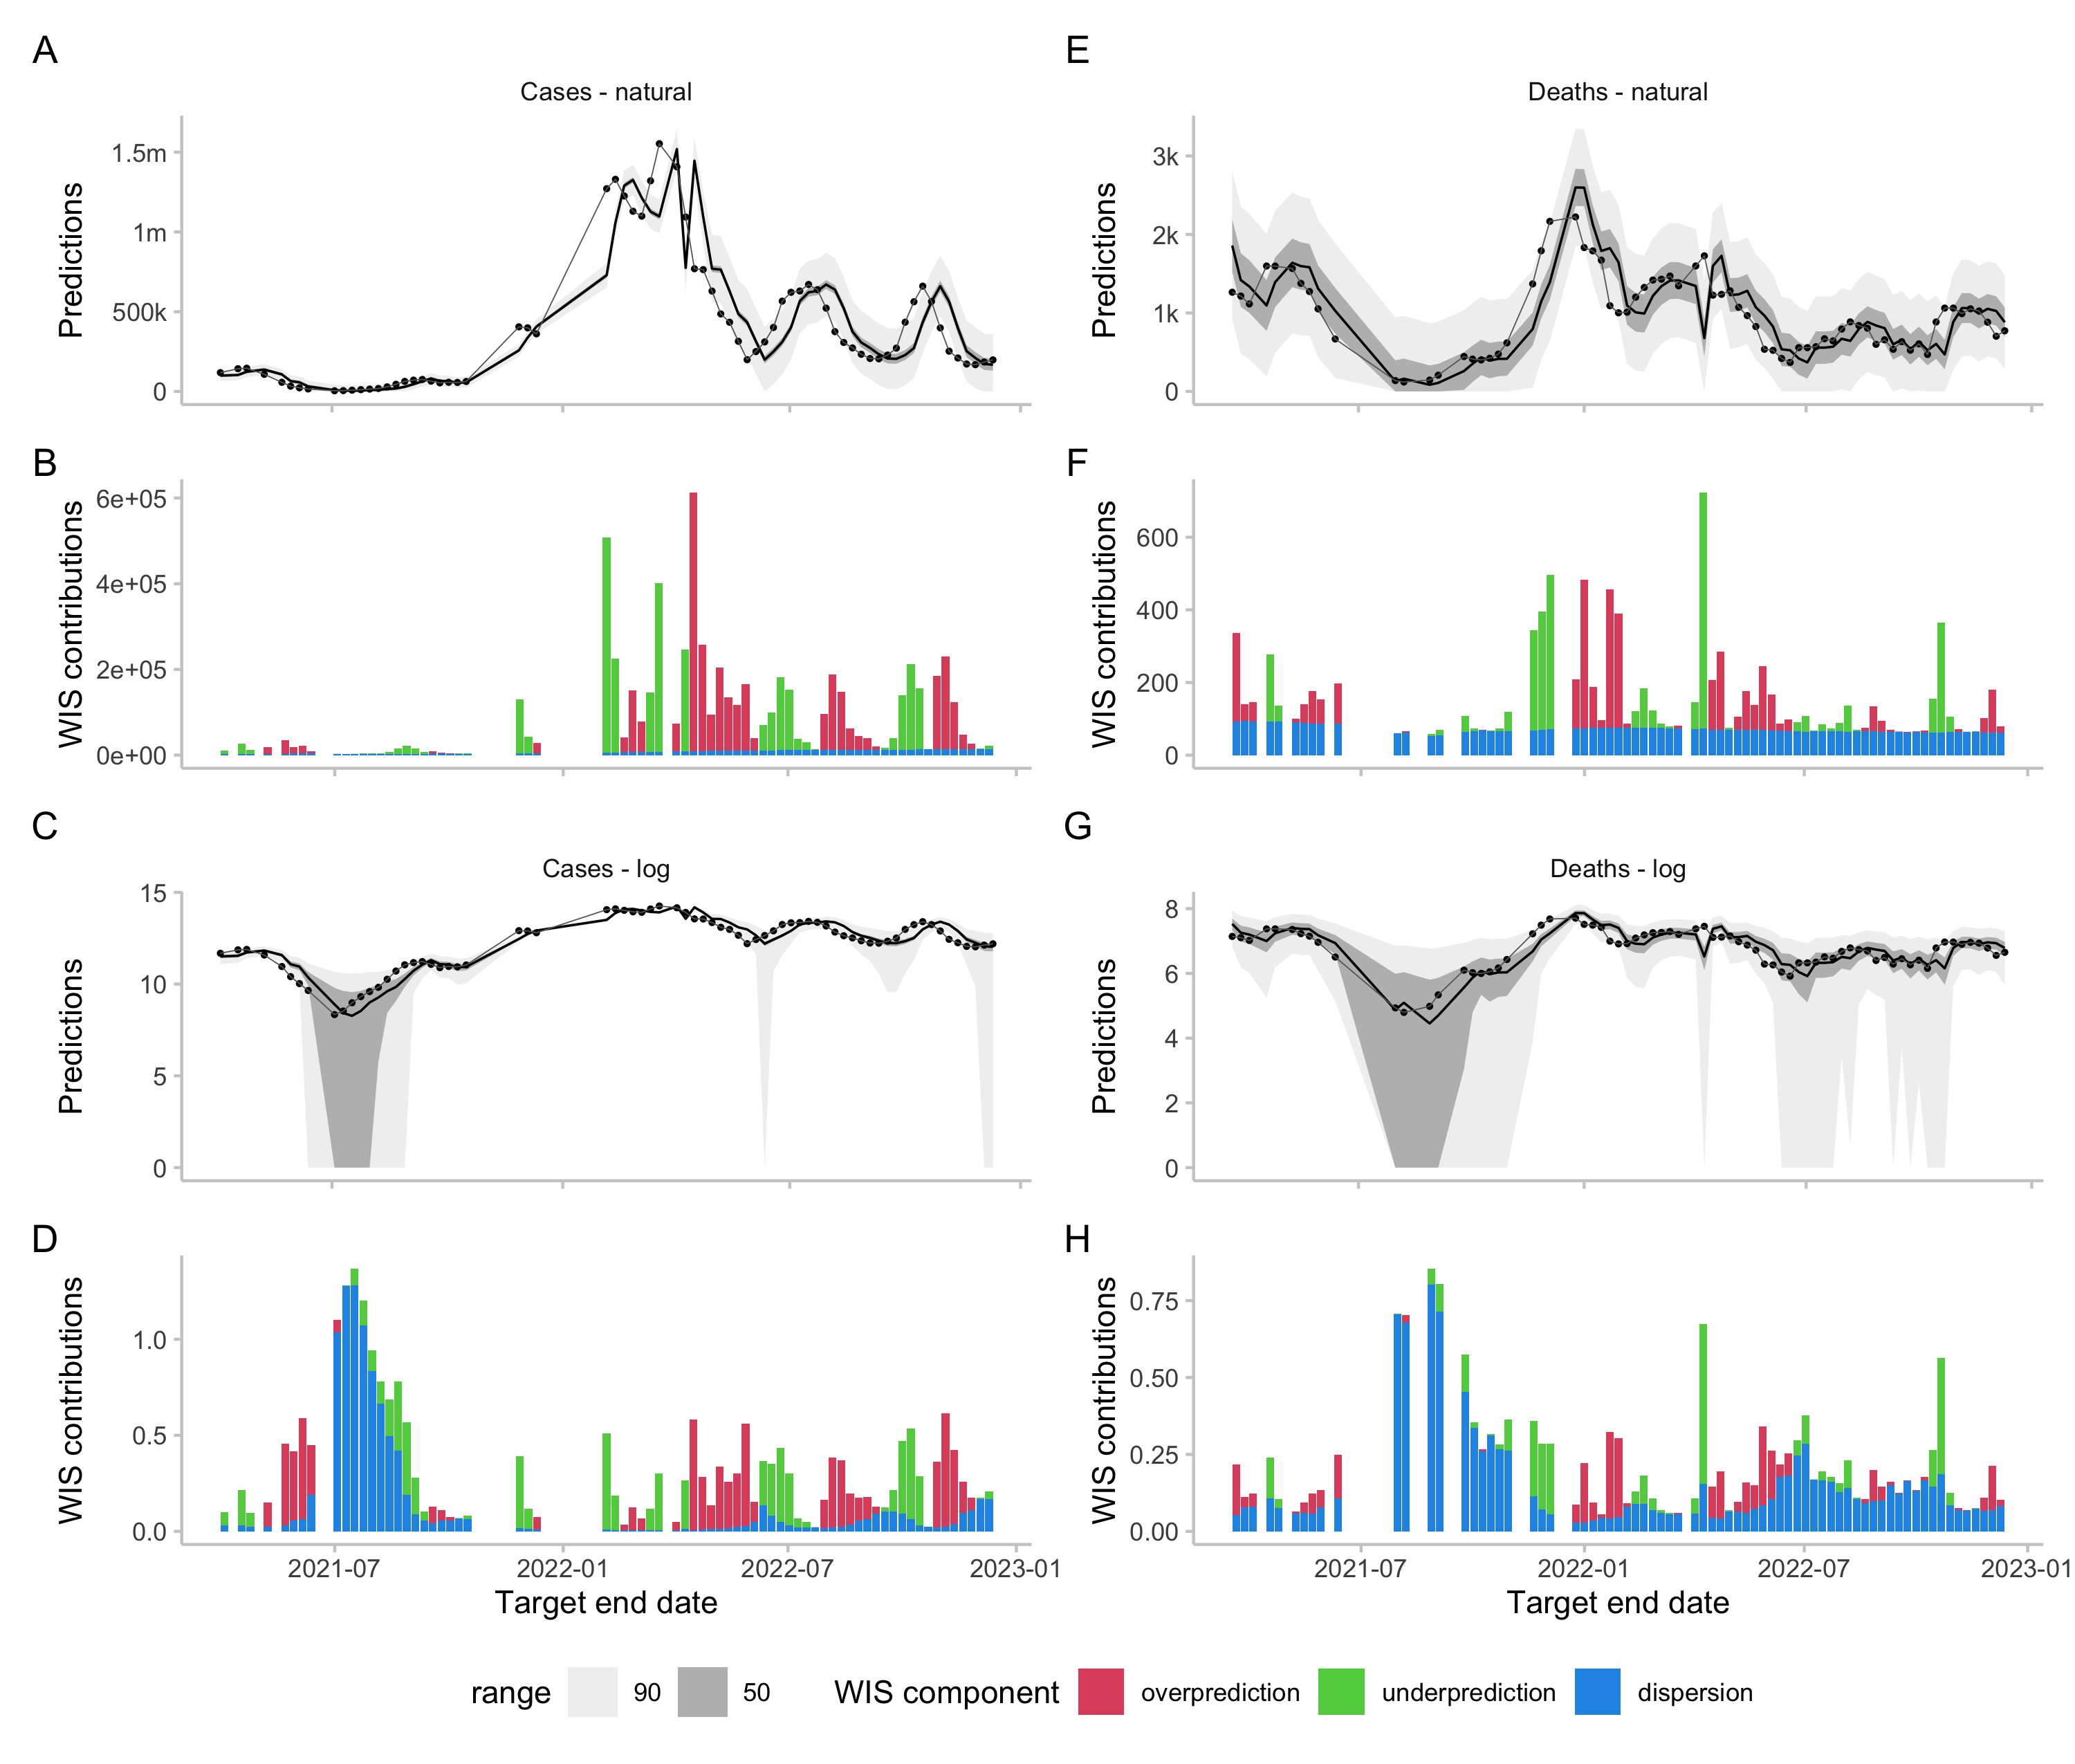
\includegraphics[width=0.99\textwidth]{output/figures/HUB-model-comparison-baseline.png}
    \caption{
    Forecasts and scores for two-week-ahead predictions from the EuroCOVIDhub-baseline made in Germany. The model had zero included in some of its 50 percent intervals (e.g. for case forecasts in July), leading to excessive dispersion values on the log scale. One could argue that including zero in the prediction intervals constituted an unreasonable forecast that was rightly penalised, but in general care has to be taken with small numbers. A, E: 50\% and 90\% prediction intervals and observed values for cases and deaths on the natural scale. B, F: Corresponding scores. C, G: Forecasts and observations on the log scale. D, H: Corresponding scores. 
    }
    \label{fig:HUB-model-comparison-baseline}
\end{figure}

\begin{figure}[h!]
    \centering
    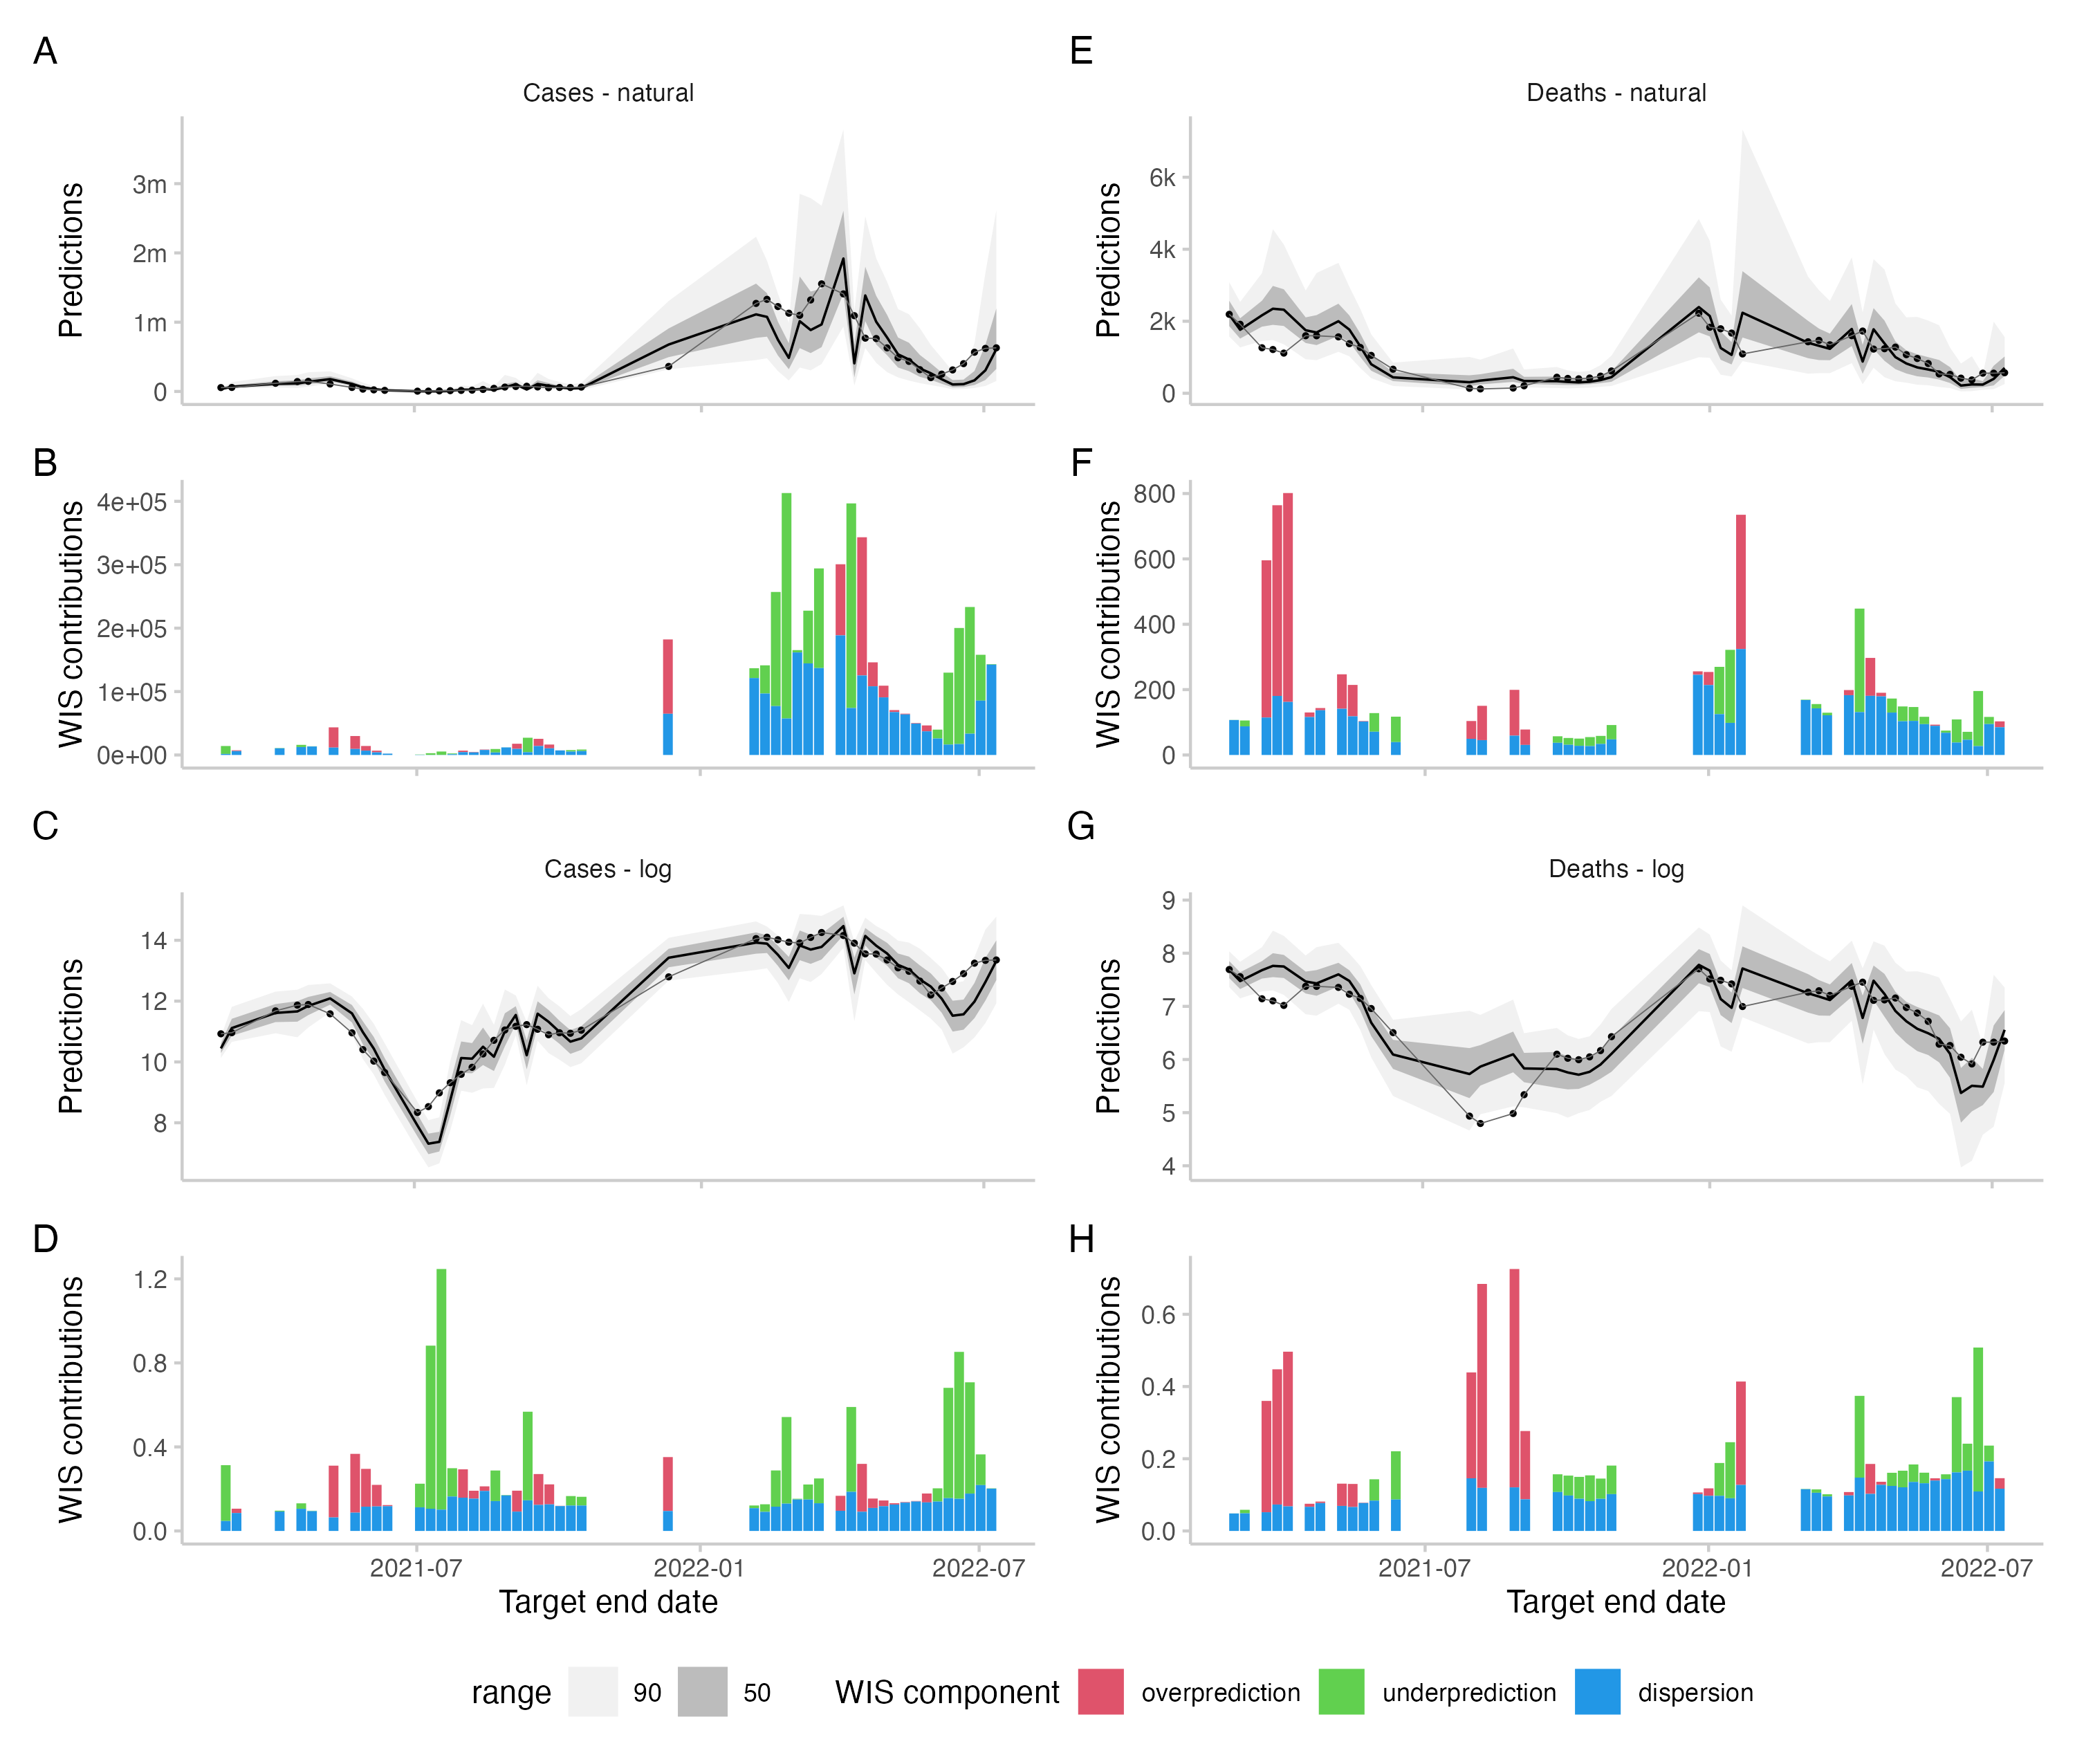
\includegraphics[width=0.99\textwidth]{output/figures/HUB-model-comparison-epinow.png}
    \caption{
    Forecasts and scores for two-week-ahead predictions from the epiforecasts-EpiNow2 model made in Germany. A, E: 50\% and 90\% prediction intervals and observed values for cases and deaths on the natural scale. B, F: Corresponding scores. C, G: Forecasts and observations on the log scale. D, H: Corresponding scores. 
    }
    \label{fig:HUB-model-comparison-epinow}
\end{figure}


\begin{figure}[h!]
    \centering
    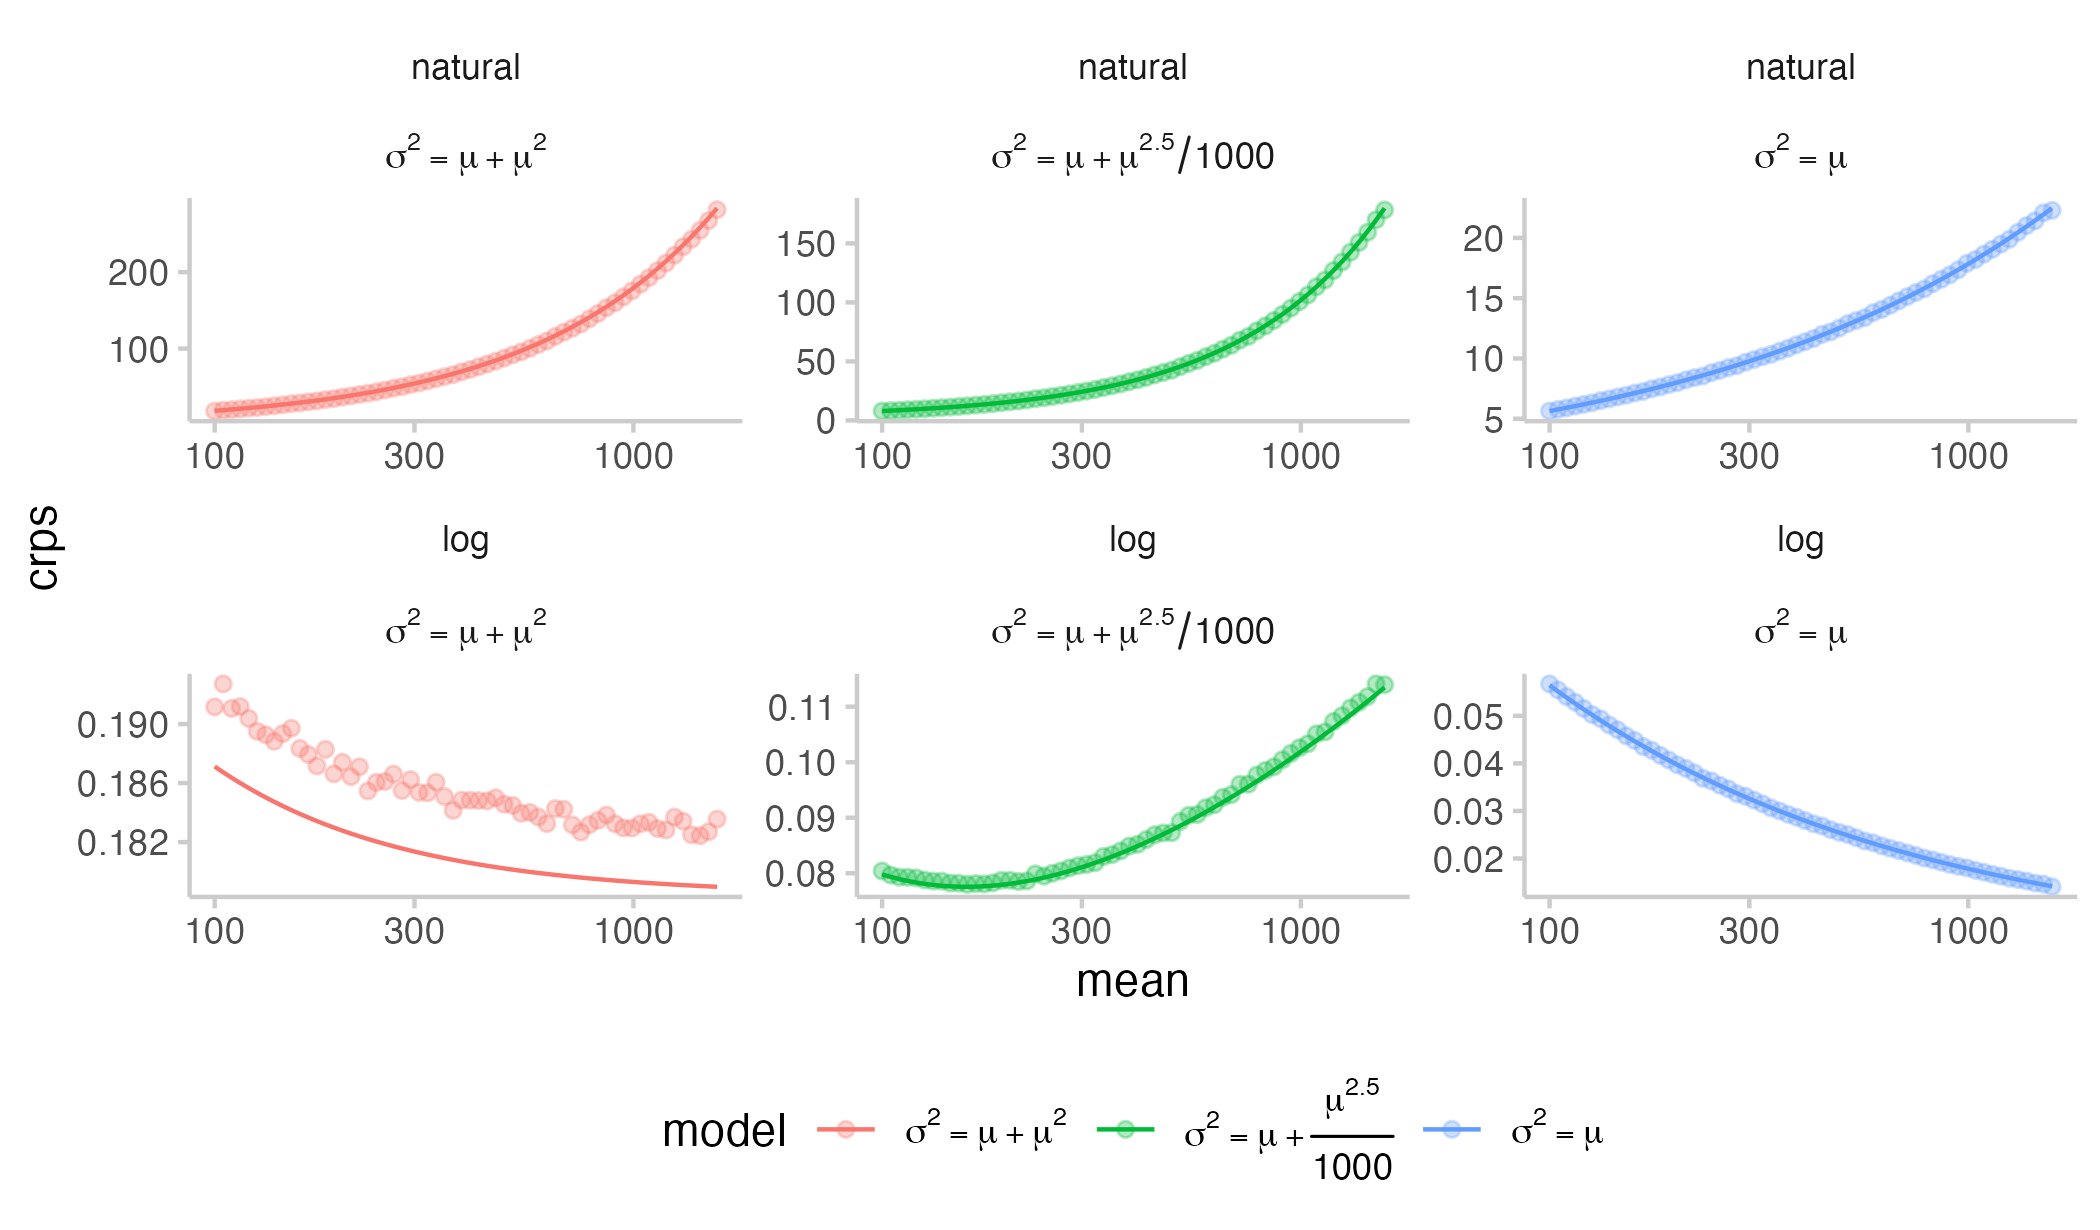
\includegraphics[width=0.99\textwidth]{output/figures/SIM-score-approximation.png}
    \caption{
    Visualisation of expected CRPS values against approximated scores using the approximation detailed in Section \ref{sec:methods:rankings} (see also Figure \ref{fig:SIM-wis-state-size-mean}). Expected CRPS scores are shown for three different distributions once on the natural scale (top row) and once scored on the log scale (bottom row).  
    }
    \label{fig:HUB-model-comparison-epinow}
\end{figure}


\begin{table}
\centering
\begin{tabular}{ccrrrrrr}
\toprule
Horizon & Target & $\alpha$ & $\beta$ & $\alpha_{\log}$ & $\beta_{\log}$ & $\alpha_{\sqrt{\ }}$ & $\beta_{\sqrt{\ }}$\\
\midrule
all & all & -1.093 & 0.963 & 0.390 & 0.001 & -0.995 & 0.209\\
\addlinespace
all & Cases & 0.036 & 0.858 & 0.751 & -0.033 & 0.047 & 0.201\\
all & Deaths & -0.885 & 0.868 & 0.430 & -0.021 & -7.564 & 0.826\\
\addlinespace
1 & all & -1.402 & 0.923 & 0.318 & -0.014 & 0.318 & 0.088\\
2 & all & -1.221 & 0.967 & 0.364 & -0.003 & 0.111 & 0.164\\
3 & all & -1.001 & 0.984 & 0.408 & 0.008 & -1.283 & 0.255\\
4 & all & -0.757 & 0.986 & 0.467 & 0.016 & -1.041 & 0.312\\
\addlinespace
1 & Cases & -0.861 & 0.876 & 0.433 & -0.024 & 0.785 & 0.087\\
2 & Cases & -0.243 & 0.877 & 0.660 & -0.031 & 0.959 & 0.162\\
3 & Cases & 0.372 & 0.855 & 0.882 & -0.037 & 1.115 & 0.238\\
4 & Cases & 0.816 & 0.837 & 1.009 & -0.036 & 1.665 & 0.296\\
\addlinespace
1 & Deaths & -1.145 & 0.831 & 0.376 & -0.035 & 0.458 & 0.048\\
2 & Deaths & -0.980 & 0.866 & 0.415 & -0.027 & 0.445 & 0.084\\
3 & Deaths & -0.809 & 0.885 & 0.441 & -0.016 & -8.262 & 0.903\\
4 & Deaths & -0.603 & 0.891 & 0.488 & -0.007 & -7.834 & 0.898\\
\bottomrule
\end{tabular}
\caption{Coefficients of three regressions for the effect of the magnitude of the median forecast on expected scores. The first regression was 
$\log[\text{CRPS}(F, y)] = \alpha + \beta \times \log[\text{median}(F)], $ where $F$ is the predictive distribution and $y$ the observed value. The second one was 
$\text{CRPS}(F_{\log}, \log y) = \alpha_{\log} + \beta_{\log} \cdot \log{(\text{median}(F))},$ where $F_{\log}$ is the predictive distribution for $\log y$. The third one was $\text{CRPS}(F_{\sqrt{\ }}, \sqrt{y}) = \alpha_{sqrt{\ }} + \beta_{sqrt{\ }} \cdot \sqrt{(\text{median}(F))},$ where $F_{\sqrt{\ }}$ is the predictive distribution for $\sqrt{y}$.
}
\label{tab:HUB-regression}
\end{table}




\clearpage
\bibliography{log-or-not.bib}


\end{document}